\documentclass[../main.tex]{subfiles}
\graphicspath{{\subfix{../images/}}}
\begin{document}
\section{Experiments and results}

In this section we are going to present the experiments and results obtained with the developed turn-taking module both in terms of performance of the system and accuracy. In particular this section is divided into four subsections that are:  "Model's inference latency" where we do an analysis of the latency introduced by the model inference; "End of turn detection latency" where we talk about how we measure the latency of the system in detecting the end of turn; "System throughput" where we talk about the throughput of the system and "Performance metrics" where we make a comprehensive analysis of the system accuracy in detecting voice in different scenarios, using different datasets and audio manipulation to add background noises. This last section will also present a comparison between the performances of the system using the Silero vad and the WebRTC vad component. The section will be divided in three subsections: "Libri-Demand dataset" where we will explain how we build the Libri-Demand dataset to test the system; "Test implementation" where we will discuss the implementation of the testing environment and "Results" where we will show the results obtained in terms of performance metrics. 

The experiments are performed in local. The server runs on a MacBook Air 2018 with a CPU 8 core, Neural engine 16 core and an 8 GB unified memory UMA (Unified Memory Architecture). 

\subsection{Model's inference latency}

In this section we are going to study the latency of the model's inference. This is the execution time of the processing of the audio chunk from the PyTorch model, that return the probability of the presence of voice in the audio. This latency affects the end of turn detection latency described in the next section, so it is important that it is the lowest as possible. 

The latency has been computed using the \textit{time.time()} method in the \textit{analyze()} function of the \textbf{Analyzer} class. The computed latency has been inserted in a list and the system every 200 measurements prints on screen the updated average of the latency of the inference. The listing \ref{listing:inference latency} shows the code used to compute the latency.

\begin{lstlisting}[language=Python, caption={Model's inference latency}]
tensor = torch.from_numpy(self.int2float(frame.to_ndarray()))
start_inference = time.time()
new_confidence = self.vad_model(tensor, self.sampling_rate).item()
end_inference = time.time()
inference_latency = end_inference - start_inference
self.inference_latencies.append(inference_latency)
            
# every 200 inferences the average inference latency is updated
if(len(self.inference_latencies) % 200 == 0):
    average_inference_latency = sum(self.inference_latencies) / len(self.inference_latencies)
    print(f'Average inference latency is {average_inference_latency} computed over {len(self.inference_latencies)} measurements')
\end{lstlisting}
\label{listing:inference latency}

The experiments are done using different sampling rate and frames duration. The results obtained are shown in the table \ref{tab:inference time}. It shows the average inference time computed over 3000 measurements.

\begin{table}[ht]
    \centering
    \begin{tabular}{|l|c|c|} \hline 
         Duration (ms)& 8 kHz &16kHz\\ \hline 
         40&  5.89&5.84\\ \hline 
         50&  6.00&6.29\\ \hline 
         60&  8.9&6.30\\ \hline 
         80&  9.2&6.78\\ \hline 
         100&  7.82&6.87\\ \hline
    \end{tabular}
    \caption{Average inference time in ms}
    \label{tab:inference time}
\end{table}

The results obtained shows an inference time of about 6 milliseconds with very small differences depending on the frame duration and sampling rate. This processing time is negligible considering the use case of our application considering the overall latency and waiting time given by the frame transmission over internet and thresholds to wait. It seems that the different inference configurations doesn't impact the inference times, this let us choose the best configuration when we will do the accuracy analysis without impacting the performances of the system.

\subsection{End of turn detection latency}

In this section we are going to talk about how we measured the performance in terms of the latency of the system detecting the end of turn of the user. The idea is to measure how much time passes from when the user stops talking to the actual sending of the message \textit{Turn change confirmed}. This latency, together with the processing time to generate a response from the user sentence, constitutes the main parts responsible for the reactivity of the system. So the idea is to have the lower latency possible in order to minimize the response time of the system, to make the conversation as realistic as possible.

The best way to do it would be an automatic system that detects when you stop talking, takes the relative timestamps and when the system detects the turn change, measures the end timestamp to compute the latency. The problem is that to do it we would need a vad to measure another vad. This is not a good idea and another vad would introduce useless latency to the result.

Instead, we choose to measure this latency manually. In particular the idea is that, during the experiments, the user press the space bar on the Web client when he stops talking and the system automatically computes the end of turn detection latency printing it on screen. Obviously being this a manual method it is not precise in measuring the actual latency and gives an overall idea on what the responsiveness of the system is. 

In particular this is obtained getting the timestamp on the JavaScript client of when the space bar is pressed. Then this timestamp is passed to the Server thought a WebRTC Data channel. This received timestamp is then saved in the Analyzer object and will be compared with the timestamp obtained in the moment of the actual sending of the \textit{Turn changed confirmed} message, that is when the actual turn change happens in the \textit{set\_state()} method. The listing \ref{listing:client latency} shows the simple JavaScript code on the client while the listing \ref{listing:server latency} shown how the message on the data channel in handled on the server.

\begin{lstlisting}[language=JavaScript, caption={Client implementation of the method to take the timestamp}]
// Add an event listener to the document for the keydown event
document.addEventListener('keydown', function(event) {
    // Check if the pressed key is the space bar (key " ")
    if (event.key === " ") {
        end_of_turn = Date.now();
        //send the time over the data streaming
        dc.send(end_of_turn);
    }
});
\end{lstlisting}
\label{listing:client latency}

\begin{lstlisting}[language=Python, caption={Server handling of the client timestamp}]
@pc.on("datachannel")
    def on_datachannel(channel):
        @channel.on("message")
        def on_message(message):
            analyzer.end_of_turn_timestamp = int(message)
\end{lstlisting}
\label{listing:server latency}

Even if we know that this method is not very precise, in order to give an indicative overview of the latency introduced by the system in this work we tried to make an experiment to provide an indicative value for the latency. The experiment consisted in taking 30 measurement and considering the average value as the latency of the system. In particular the obtained value was of 796 ms with a \textit{confirmed\_silence\_threshold} of 700 ms. This means that the system would have an ideal latency of 700 ms because it has to wait at least the \textit{confirmed\_silence\_threshold} to confirm the end of turn detection, while our system introduces 96 ms of difference from this value. In the end considering the order of magnitude of the ideal latency the system provide a good result in terms of the additional latency introduced since it adds a latency that is the 14 \% of the ideal value. It is important to consider that the experiment is performed locally and brings an additional latency that is coherent with the type of operations done by the system, as for example the buffering created by WebRTC. 

\subsection{System throughput}

In this section we are going to talk about the throughput of the system, that is how many audio chunks the system is able to process in a given period of time. The obvious idea is that the system should process the frames at a higher rate with respect to the rate at which they arrive, avoiding creating a buffer of incoming frames to process. 

In particular, we measure the time that passes from one audio frame processing to the other, that is the rate at which the system updates the state of the communication. This is done simply taking the timestamp at which the last state is updated and comparing it with the last timestamp taken. The average of this value is then updated every 100 processing. The implementation is found in the listing \ref{listing:throughput implementation}

\begin{lstlisting}[language=Python, caption={System throughput analysis implementation}]
new_end_analyze = time.time()
gap = new_end_analyze - self.old_end_analyze
if self.old_end_analyze != 0:
    self.analyze_gaps.append(gap)
    print(f'Analyze gap: {gap}')
self.old_end_analyze = new_end_analyze
if(len(self.analyze_gaps) > 0 and len(self.analyze_gaps) % 100 == 0):
    average_analyze_gap = sum(self.analyze_gaps) / len(self.analyze_gaps)
    print(f'Average analyze gap: {average_analyze_gap}')
\end{lstlisting}
\label{listing:throughput implementation}

The results obtained about the single "analyze gaps", that is the time gap between two processing, depends on the value of the frame duration specified in the configuration file while the average analyze gap is very near the ideal value of the frame duration parameter. In particular if for example the frame duration parameter is 40 ms the single analyze gaps and the average analyze gap is near that value while if the frame duration parameter is 50 ms the single analyze gaps are between 40 ms and 60 ms with the average value that is very near the 50ms ideal value. This happens because the audio frames coming from WebRTC has a standard duration of 20 ms and in order to process them we collect them in a FIFO buffer until we have all the samples for the desired frame duration. This means that in order to process the first audio frame we have to wait 3 packets of 20 ms each waiting in total 60 ms. Once we process the 50 ms audio frame we have to wait "only" other 2 packets this time for a total of 40 ms because we have already stored 10 ms of audio samples in the buffer. The next time we have to wait again 60 ms and so on. This happens only when the frame duration in not a multiple of 20 ms. When that is the case we have only to wait the correct number of packets because we are going to use them all. For example with a frame duration of 40 ms every time we need to wait 2 packets of 20 ms each that arrive from WebRTC and we can continue with the processing immediately. 

Regarding the average analyze gap instead the value is really near the ideal value of the frame duration parameter. For example in an experiment with the frame duration at 50 ms the average analyze gap value computed over 300 measurements is of 49.78 ms. In a second experiment with the frame duration value of 40 ms the average analyze gap computed over 300 measurements was of 39.73 ms. 

\subsection{Performance metrics}

In this section we are going to present the testing performed on the system in order to obtain the performance metrics such as: accuracy, precision, recall and f1-score of the system comparing the results obtained using both the silero vad and the WebRTC vad.

\subsubsection{Libri-Demand dataset}

In this section we will explain the details of the dataset used for testing the performances of the system and the procedure of how we created it.

In order to accurately test the performances of the system and in particular of the voice activity detection part, we would need a dataset composed of different spoken audio parts with various types of background noises in different environment and different noise levels. Since we didn't find an available audio dataset meeting our requirements we decided to create our own dataset and we called it Libri-Demand dataset. It is called this way because it is derived from the LibriSpeech and DEMAND datasets applying different elaborations and intersections. The dataset contains 12.2 hours of noisy speech both with male and female voices with a background noise of 17 different categories. The dataset size is of 1.54 GB and contains the audio data in the WAV format with a sampling rate of 16kHz.

The LibriSpeech dataset is a corpus of approximately 1000 hours of 16kHz read English speech. The data is derived from read audiobooks from the LibriVox project, and has been carefully segmented and aligned. The corpus is split into several parts to enable users to selectively download subsets of it, according to their needs. The subsets with "clean" in their name are supposedly "cleaner"(at least on average), than the rest of the audio and US English accented. We used the "test-clean" part for our purpose since we needed clean speech audio to merge with noisy audio to create our noisy dataset. The corpus come with three label files: SPEAKERS.txt, CHAPTERS.txt and BOOKS.txt. The first file contains the following information:

\begin{itemize}
    \item reader\_id: the ID of the reader in the LibriVox's database
    \item gender: 'F' for female, 'M' for male
    \item subset: the corpus subset to which the reader's audio is assigned
    \item duration: total number of minutes of speech by the reader, included in the corpus
    \item name: the name under which the reader is registered in LibriVox
\end{itemize}

The second file contains the following information regarding the chapters read in the corpus:

\begin{itemize}
    \item chapter\_id: the ID of the chapter in the LibriVox's database
    \item reader\_id: the ID of the reader in the LibriVox's database
    \item duration: how many minutes of this chapter are used in the corpus
    \item subset: the corpus subset to which this chapter is assigned
    \item project\_id: the LibriVox project ID
    \item book\_id: the Project Gutenberg's ID for the book on which the LibriVox project is based
    \item chapter\_title: the title of the chapter on LibriVox
    \item project\_title: the title of the LibriVox project
\end{itemize}

Finally, the last file contains a list of the books from which the chapters are taken.

The DEMAND dataset is the dataset from which we have taken the background noises to merge with the clean speech. This dataset is a collection of multichannel recordings of acoustic noise in diverse environments and it aims to provide a set of recordings that allow testing of algorithms using real-world noise in a variety of settings. All recordings are made with a 16-channel array but since our testing needed mono audio we used only the first channel. The current database is divided into 6 categories, 4 of which are “inside” and 2 of which are open air.
The inside environments are classified as Domestic, Office, Public, and Transportation; the open air environments are Street and Nature.

In the “Domestic” category, the recordings are:

\begin{itemize}
    \item \textbf{DWASHING} inside a washroom with a front-loading washer running a wash cycle
    \item \textbf{DKITCHEN} inside a kitchen during the preparation of food
    \item \textbf{DLIVING} inside a living room
\end{itemize}

The “Nature” category has three outdoor environment recordings:

\begin{itemize}
    \item \textbf{NFIELD} a sports field with activity nearby
    \item \textbf{NRIVER} a creek of running water
    \item \textbf{NPARK} a well-visited city park
\end{itemize}

In the “Office” category, the recordings are:

\begin{itemize}
    \item \textbf{OOFFICE} a small office with a three people using computers
    \item \textbf{OHALLWAY} a hallway inside an office building, with individuals and groups passing by
    occasionally
    \item \textbf{OMEETING} a meeting room while the microphone array is discussed
\end{itemize}

In the category “Public”, recordings are of interior public spaces:

\begin{itemize}
    \item \textbf{PSTATION} the main transfer area of a busy subway station
    \item \textbf{PCAFETER} a busy office cafeteria
    \item \textbf{PRESTO} a university restaurant at lunchtime
\end{itemize}

The “Street” category has outdoor recordings made near inner-city public roads:

\begin{itemize}
    \item {STRAFFIC} a busy traffic intersection
    \item \textbf{SPSQUARE} a public town square with many tourists
\end{itemize}

“Transportation” describes a set of recordings made in the inside of vehicles:

\begin{itemize}
    \item \textbf{TMETRO} a subway
    \item \textbf{TBUS} a public transit bus
    \item \textbf{TCAR} a private passenger vehicle
\end{itemize}

Recordings were made at 48 kHz for a long duration then trimmed to 300 s to avoid setup noises that are not part of the “natural” background noise. The data is available both at the original sampling rate and downsampled to 16 kHz. For the dataset we used the 16kHz sampling rate to match sampling rate of the spoken audio from the LibriSpeech dataset.

The Libri-Demand dataset is composed of 6 parts: male clean, female clean, male noisy, female noisy, noisy sessions clean and noisy sessions noise. The male clean and female clean parts contains clean speech from the LibriSpeech dataset combined to obtain 10 sessions of the duration of 3 minutes for each part, for a total of 1 hour of clean speech. These sessions are obtained combining random different sessions taken from the LibriSpeech dataset separated by artificial silence of a random duration between 2.1 and 3.0 seconds. The metadata of these sessions contains the ID of the session, the list of the files with the utterances contained in the session, the list of spoken parts delimited by a "start" and "stop" timestamp, the noise file that contains the noise applied to the session (for these clean parts this value is "none"), the SNR level, used in the noisy datasets here it is leaved to zero and the clean session field used during the construction of the noisy dataset is leaved as "none". An example of session metadata is shown in Figure \ref*{fig:session_clean} (the lists are interrupted with "..." for space reasons). A further explanation on the implementation on how this dataset is build can be found in the next part.

\begin{figure}[ht]
    \centering
    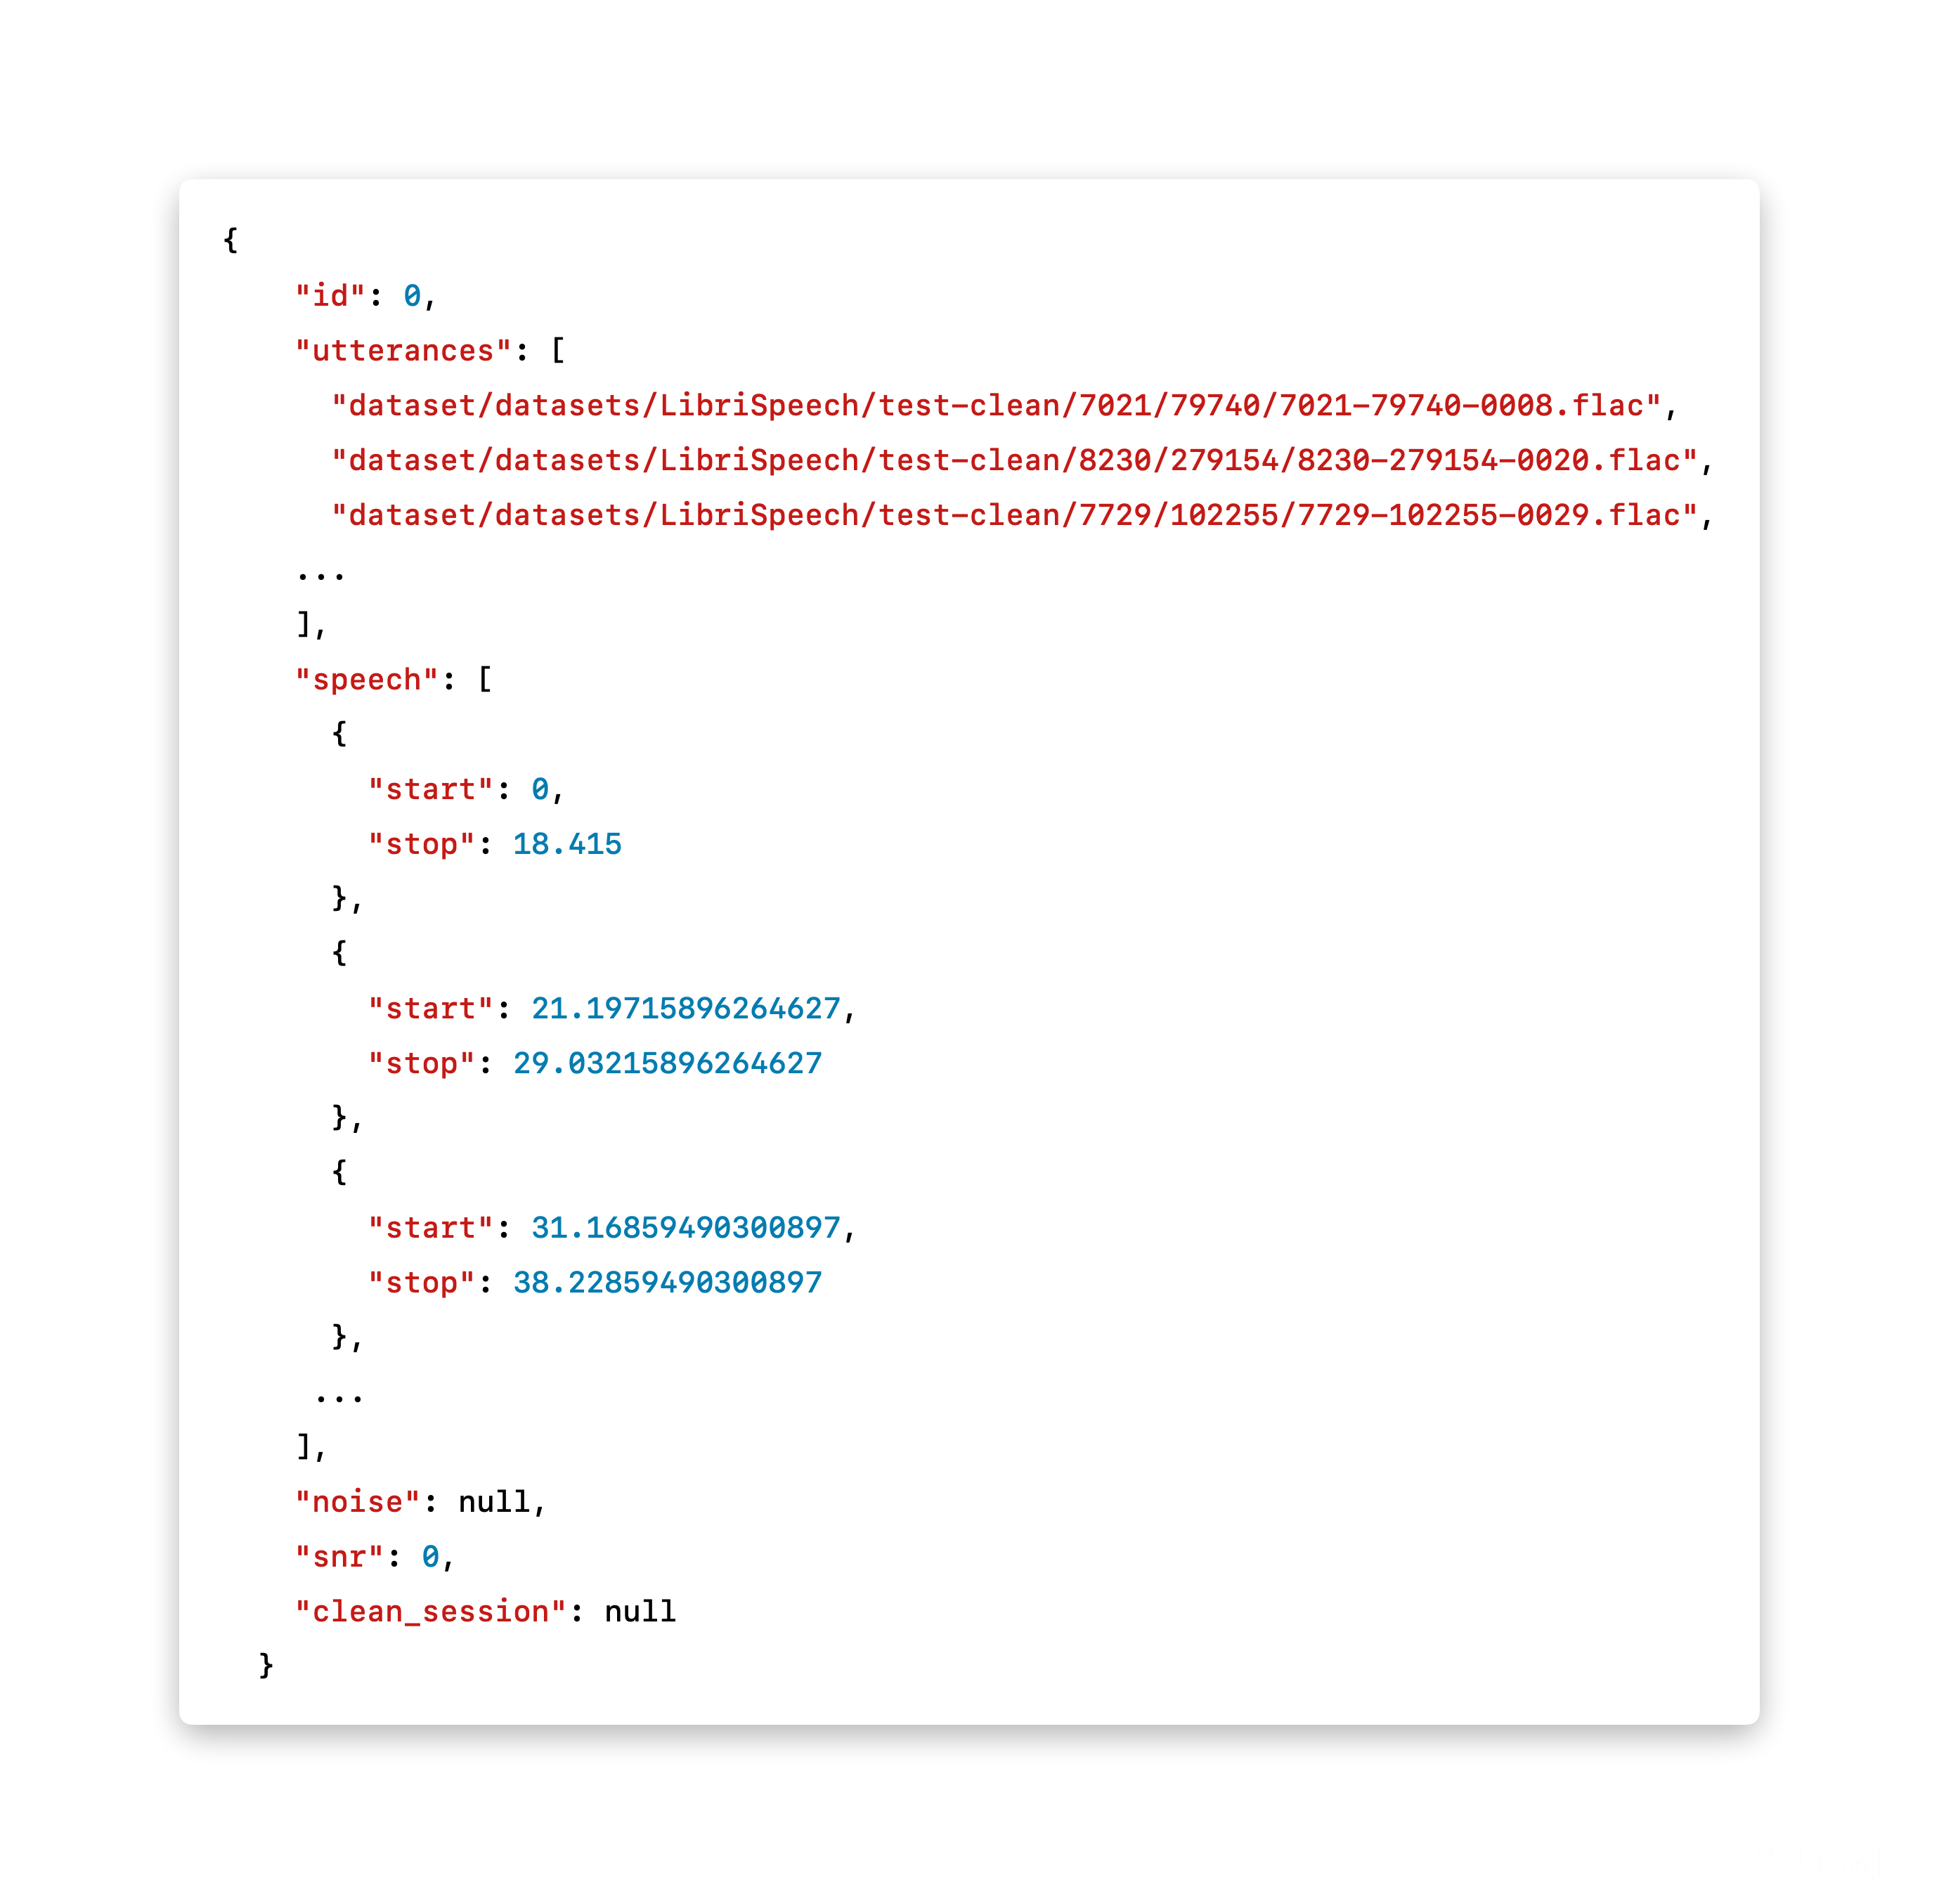
\includegraphics[width=\textwidth]{images/session_clean.png}
    \caption{Male clean metadata}
    \label{fig:session_clean}
\end{figure}

In order to effectively test the performance of the system and in particular the vad part, we needed audio data with speech and background noise. So we added the noises from the DEMAND dataset to the male clean and female clean part obtaining the male noisy and female noisy parts of our dataset. In particular three random sessions extracted from the clean sessions where merged with the 17 different categories of noise sources obtaining 51 noisy sessions, both for male and female audio data, obtaining in total 102 sessions long 3 minutes, for a total of 5.1 hours of noisy speech. Since we wanted to normalize the level of spoken and noisy audio we decided to apply the noise with an SNR of 0db obtaining very noisy sessions where the level of speech was the same as the level of noise. 

The signal-to-noise ratio (SNR) is a measure used in various fields, including electronics, telecommunications, and data analysis, to quantify the strength or quality of a signal in relation to the surrounding background noise. It is expressed as the ratio of the amplitude or power of the signal to the amplitude or power of the noise. The SNR is calculated using the following formula:

\[ SNR = \frac{Signal Power}{Noise Power} \]
 
In decibels (dB), the formula is often expressed as:

\[ SNR_{{dB}} = 10 \cdot \log_{10}\left(\frac{Signal Power}{Noise Power}\right) \]


A higher SNR indicates a stronger and more reliable signal relative to the background noise. A lower SNR, on the other hand, suggests a higher level of noise compared to the signal, making it more challenging to extract meaningful information from the data.

In Figure \ref*{fig:session_noisy} is shown an example of metadata for the male noisy session. The labels are the same of the male clean metadata but here the noise field contains the actual file from which the applied noise was taken and the clean sessions from which the clean speech was taken. 

\begin{figure}[ht]
    \centering
    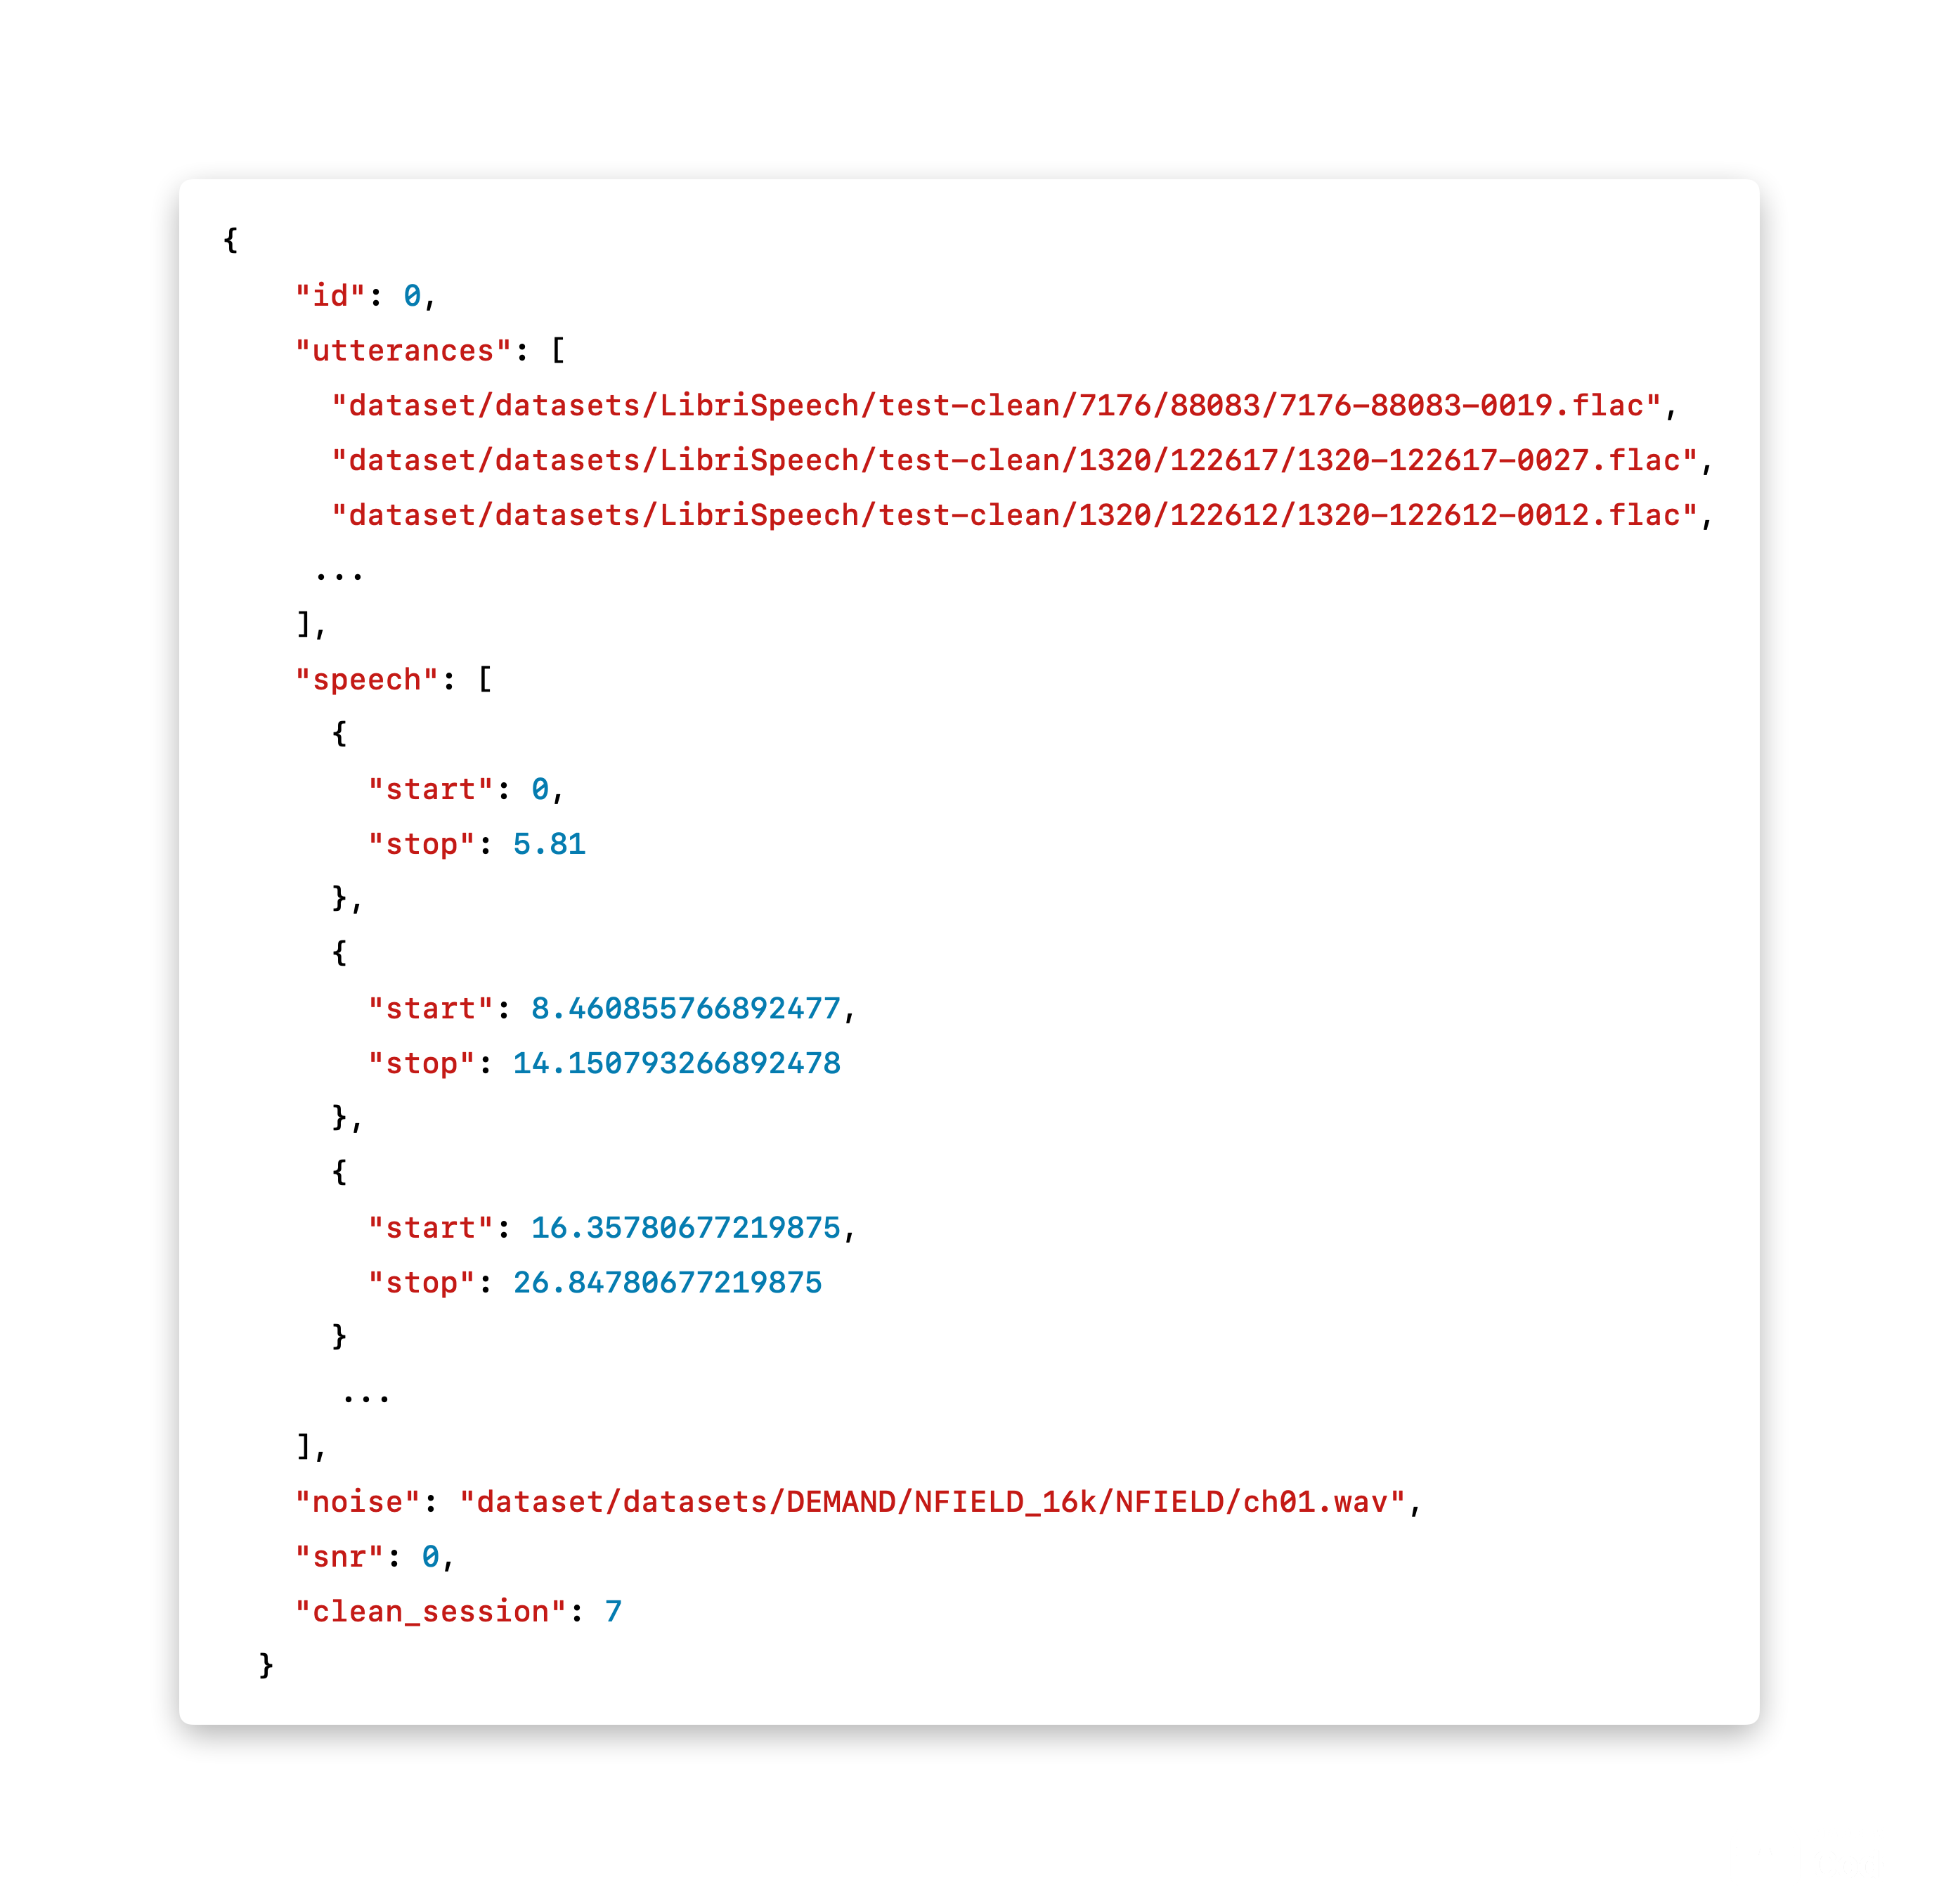
\includegraphics[width=\textwidth]{images/session_noisy.png}
    \caption{Male noisy metadata}
    \label{fig:session_noisy}
\end{figure}

For our testing purposes we wanted also to compute the performance metrics on noisy audio with different SNR. For this reason we created the noisy sessions part that is made up of one single clean speech session to which is applied all the 17 categories of noise with 5 different SNR: 20db, 10db, 0db, -10db, -20db. The clean session used for the whole part is always the same and it is generated with both male and female random voices for a duration of 5 minutes. In this part there are 85 different sessions and the total duration of this part is 5 minutes for session for 17 categories for 5 different SNR levels for a total of 425 minutes or 7 hours of noisy speech. The noisy sessions metadata is the same for the male noisy metadata with the SNR field that varies for the different levels. In total the Libri-Demand dataset contains more than 12 hours of noisy speech.

Regarding the implementation of the construction of the Libri-Demand dataset it has been done in 2 parts: the creation of the metadata and the creation of the dataset from the metadata. 

The creation of the metadata is contained in the create\_metadata.py file. First we read all the IDs of the speakers from the SPEAKERS.txt file of the LibriSpeech dataset described before, we get all the utterances name files present in the LibriSpeech dataset, and then we separate the utterances by gender in order to obtain a list of file names containing male and female utterances. To obtain the clean sessions we passed each list to the \textit{create\_clean\_sessions()} method passing as argument the list of utterances obtained before. Here a list of Sessions is created choosing randomly selected utterances from the passed list adding after each utterance a chunk of silence of random duration between 2.1 and 3 seconds, until the duration of the session reached at least 3 minutes. The duration of each utterance was obtained using the \textit{librosa.get\_duration()} method of the \textbf{librosa} module. The obtained list of Sessions was then written to a json file since it is the metadata of the clean part. 

To create the noisy sessions we get the list of the noise files with the \textit{get\_noises()} method and we pass them with the male and female sessions to the \textit{create\_noisy\_sessions()} method. It chooses at random 3 sessions from the passed list and for each one it creates a new session for each noise file found in the noises list, that will be specified in the noise label of the metadata. This way we obtain our 51 sessions per gender and we write it to the correct metadata json file. The implementation of the \textit{create\_noisy\_sessions()} is shown in listing \ref{listing:create_noisy_sessions}

\begin{lstlisting}[language=Python, caption={create\_noisy\_sessions()}]
    def create_noisy_sessions(sessions, noises):
        picks = []
        pick = None
        noisy_sessions = []
        Session.session_counter = 0
        for i in range(CLEAN_PICKS):       
            while pick == None or pick in picks:
                pick = random.randint(0, len(sessions) - 1)
            picks.append(pick)
            session = sessions[pick]
            for noise in noises:
                noisy_session = Session(session.utterances, session.speech, noise, clean_session=session.id)
                noisy_sessions.append(noisy_session)
            
        return noisy_sessions
    \end{lstlisting}
    \label{listing:create_noisy_sessions}

Finally, to create the noisy sessions with different SNR levels first we create a new clean session of the duration of 5 minutes taking randomly the utterances from both the male and female list, then we create a new Session for each noise and for each noise level specifying in the constructor of the \textbf{Session} class the noise, the SNR and always the same clean session. 

Once we defined the metadata files, we created the dataset starting from them. We can find the implementation of this procedure in the create\_dataset.py file. To create the clean datasets first we read the metadata json files to obtain the information about the sessions to create. These sessions are passed to the \textit{create\_clean\_dataset()} method. This method uses the \textbf{AudioSegment} object from the \textbf{pydub} module to create a new audio data. In particular, we use the \textit{AudioSegment.from\_file()} function to create a new audio session starting from the first utterance found in the utterances list of the session that we are creating. We then add a silence part thanks to the \textit{AudioSegment.silent()} method passing as argument the silence duration in milliseconds, that we obtain from the speech chunks information present in the metadata. Once we summed all utterance of a session and the relative silences we save the new sessions in the WAV format thanks to the \textit{AudioSegment.export()} method. The \textit{create\_clean\_dataset()} method is shown in listing \ref{listing:create_clean_dataset}

\begin{lstlisting}[language=Python, caption={create\_clean\_dataset()}]
def create_clean_dataset(output_path, sessions):
    for session in sessions:
        output_file = output_path + "session_" + str(session.id) + ".wav"
        audio_session = AudioSegment.silent(0, SAMPLING_RATE)

        for j, utterance in enumerate(session.utterances):
            audio_session += AudioSegment.from_file(utterance, "flac")
            if j+1 != len(session.utterances):
                silence_duration = session.speech[j+1]['start'] - session.speech[j]['stop']
                silence_audio = AudioSegment.silent(duration=silence_duration * 1000, frame_rate=SAMPLING_RATE)
                audio_session += silence_audio
        
        audio_session.export(output_file, format="wav")
\end{lstlisting}
\label{listing:create_clean_dataset}

To create the noisy dataset we operate similarly, but this time we need to add the background noise with the correct SNR. This last operation is performed in the \textit{join\_audio()} function, called from the \textit{create\_noisy\_dataset()} function, taking as inputs the path of the clean session, the path of the noise and the SNR level. In this function the clean and the noise signals are loaded as arrays the power of them is computed. Then the normalization and the procedure to scale the noise power to obtain the correct SNR is applied. Finally, the mixed array is saved as a wave file using the \textbf{wave} module.

In the end to create the noisy sessions with different SNR levels we reuse the same methods used before to create the desired clean session that will be mixed with the noises with the specified noise level in the metadata file.

\subsubsection{Test implementation}

In this section we are going to present how the system was tested to obtain the performance metrics using the libri-demand dataset. The idea is to test the voice activity detection part of the system comparing the results obtained using as vad part the Silero vad and the WebRTC vad. The Libri-Demand dataset will be sent from the client of the application and the server will process the incoming audio writing to a file the spoken segments contained in each session. The results will be then compared to the metadata containing the ground truth obtaining the classical performance metrics of a classification system.

We will start from the modification done to the client in order to execute the testing operation. The main difference from the normal use case of the application is that the audio that will be processed will come from an audio file and not live from a microphone. This operation is done creating a new audio element in the body of the client that will have as source the first audio file of the dataset to process. The stream of audio from the audio element will be got using the \textit{captureStream()} method of the element and the tracks of this stream will be added to the peer connection always using the \textit{addTrack()} method seen before. Once the audio session has ended a message to the server, using the peer connection data channel is sent. The server will perform the adequate operations to continue the testing in case a simple session or an entire dataset has ended and will respond with and acknowledgement message. The operations performed by the server will be explained soon. Once the client receives the acknowledgement from the server, the client loads in the audio element a new audio file that will be sent. Now the client needs to retake the stream from the audio element since the source is changed but instead of adding a new track that will change the form of the connection triggering a new connection request, the client will change the audio tracks for each sender of the connection using the \textit{replaceTrack()} method. This will keep the same connection while changing the source for the audio stream. In the listing \ref{listing:captureStream} is shown how the audio stream is obtained and how the old audio source is replaced.

\begin{lstlisting}[language=Javascript, caption={captureStream() and replaceTrack() methods}]
audioElement.oncanplay = function () {
    if (!negotiated) {
        stream = audioElement.captureStream();

        stream.getTracks().forEach(function (track) {
            pc.addTrack(track, stream);
        });
        negotiated = true;
        negotiate();
    }
    else {
        pc.getSenders().forEach(function (sender) {
            if (sender.track && sender.track.kind === 'audio') {
                sender.replaceTrack(getAudioTrack());
            }
        });
    }
}
\end{lstlisting}
\label{listing:captureStream}

In the server part we need to add the acknowledgement message on the termination of a session. We need also to modify the vad analyzer part that will keep track of the spoken parts of the incoming audio, detection that will be written on a file to be processed later. To correctly manage every session, the session termination has to be communicated by the client that needs to wait to play another session until the server is ready to receive it. This is manged using the data channel of the peer connection. The messages received by the server can be: "session\_ended" to communicate the termination of a session or "dataset\_ended" to communicate the end of an entire dataset. In both cases the called function will be the same, that is the \textit{analyzer.session\_ended()} function, but with different parameters. In both cases the server will reply with a "next\_session" message that will start the receiving of a new session from the client, eventually of a new dataset, or the receiving of the "test\_finished" message that means that the client has sent all the datasets. Another modification done to the server is that we added two arguments to the application that are the model and confidence\_threshold. The possibility of changing the model to use for detecting the audio segments allow us to use the same server to test both the system with the Silero vad and the WebRTC vad. Indeed, passing as argument the model "silero" the normal Analyzer class will be instantiated, while using the "webrtc" parameter, the server will instantiate the \textbf{AnalyzerWebRTC} object that is implemented in the vad\_analyzer\_test\_webrtc\_vad.py file. The confidence\_threshold parameter will overwrite the same parameter found in the configuration.json file, since for obtaining the results for the ROC curve we need to run the tests with different thresholds for our classifiers. 

To obtain the spoken segments for each session we modified the \textit{set\_state()} function of the vad\_analyzer\_test.py file. In particular, when the conversation starts a variable "speech\_start" is set with the current duration point of the session. When the system register the first silence frame, it sets another variable "speech\_stop" with the current point of the session. When the system register a turn change, it saves a new spoken segment saving in a list of dictionaries the two variables. In this way the start and end point of every spoken segment of the session is registered and can be compared with the one contained in the metadata. The reason why we take as spoken segment the whole turn and not only the spoken parts (in a turn there can be different spoken chunks separated by inter turn pauses) is that in the metadata we have the start and the stop of the whole utterances present in the session and not of the single parts, so we did this to match the information present in the ground truth. In the next section we will explain how the parameters were chosen based on the analysis of the LibriSpeech dataset.

Finally, lets present how we used the WebRTC vad instead of the silero vad for the tests. First, we instantiate the vad object using the \textit{Vad()} constructor of the \textbf{webrtcvad} module. We pass to the constructor the confidence\_threhsold parameter passed as argument to the server. This set its aggressiveness mode, which is an integer between 0 and 3. 0 is the least aggressive about filtering out non-speech, 3 is the most aggressive. In order to be processed by the vad, the audio frame needs to be a byte object, so we need to put it in that form transforming the frame first in a NumPy array than in a byte object using the \textit{tobytes()} method. The transformation applied is shown in listing \ref{listing:AudioFrame_trasformation}. It's important to notice that the model only works with a frame duration of 10, 20 or 30 ms, and will not work with any other frame duration.

\begin{lstlisting}[language=Python, caption={AudioFrame processing for the WebRTC vad}]
frame_array = frame.to_ndarray().astype(np.int16).squeeze()
chunk_bytes = bytes(frame_array.tobytes())
is_speech = self.vad_model.is_speech(chunk_bytes, self.sampling_rate)
\end{lstlisting}
\label{listing:AudioFrame_trasformation}

The result of the \textit{is\_speech()} method is a boolean indicating if the audio chunk is contained speech or not, differently from the Silero vad that returns a probability for the frame to contain speech.

\subsubsection{Results}

In this section we are going to present the results obtained from the computation of the performance metrics of system. First we are going to present the choices behind the parameters used in the configuration files during testing. Second we are going to present how the results are obtained from the spoken segments detected by the system. Lastly we are going to show the results in the form of: accuracy, precision, recall and f1 score obtained during testing, and we are going to compare the results obtained using the Silero vad and the WebRTC vad.

As we have discussed in the previous section that the ground truth information regarding the spoken segments in the session, contains the start and stop timestamp of the utterance in the session and not the singles spoken chunks that can be interleaved by an inter-speech pause. To match this characteristic also the system needs to detect the spoken segments as complete utterances and not single spoken chunks, avoiding confusing inter-speech pauses as the end of the utterance. This is the same problem that the system encounter in its normal use case, where it needs to distinguish a pause from an actual turn change. As we have seen in the section \ref{implementation} this is done with a threshold that tells the system when the silence can be considered a turn change and not a pause. For more details on how the system handles this threshold to detect the turn change please refer to the section \ref{vad analyzer}. In order to select the correct value for the silence threshold, we decided to analyze the LibriSpeech dataset to get some statistics on the inter-speech pauses present in the utterances of the dataset, since we were going to do the testing on those utterances. In order to do that we used the \textit{get\_speech\_timestamp()}
utility function obtained loading the silero vad model from the PyTorch Hub. This function returns a list with the start and stop timestamps of all the spoken segments contained in the audio file passed. Collecting this values and computing the pauses between these audio chunks we finally obtain a list of inter-speech pause that has been written to a file to be analyzed. Computing the quartiles and percentiles values of the pauses we found out that 90\% of the pauses have a duration shorter than 600 ms and 99\% shorter than 1100 ms. So we choose those values for the silence\_theshold and the confirmed\_silence\_threshold.

Once the test was completed, needing a little more than 12 hours, for every dataset was produced a JSON file containing a list of sessions. Every session was composed by a list of dictionaries containing start and stop timestamp of the utterances in the session. The figure \ref{fig:test-result} shows an example of the result of the testing.

\begin{figure}[ht]
    \centering
    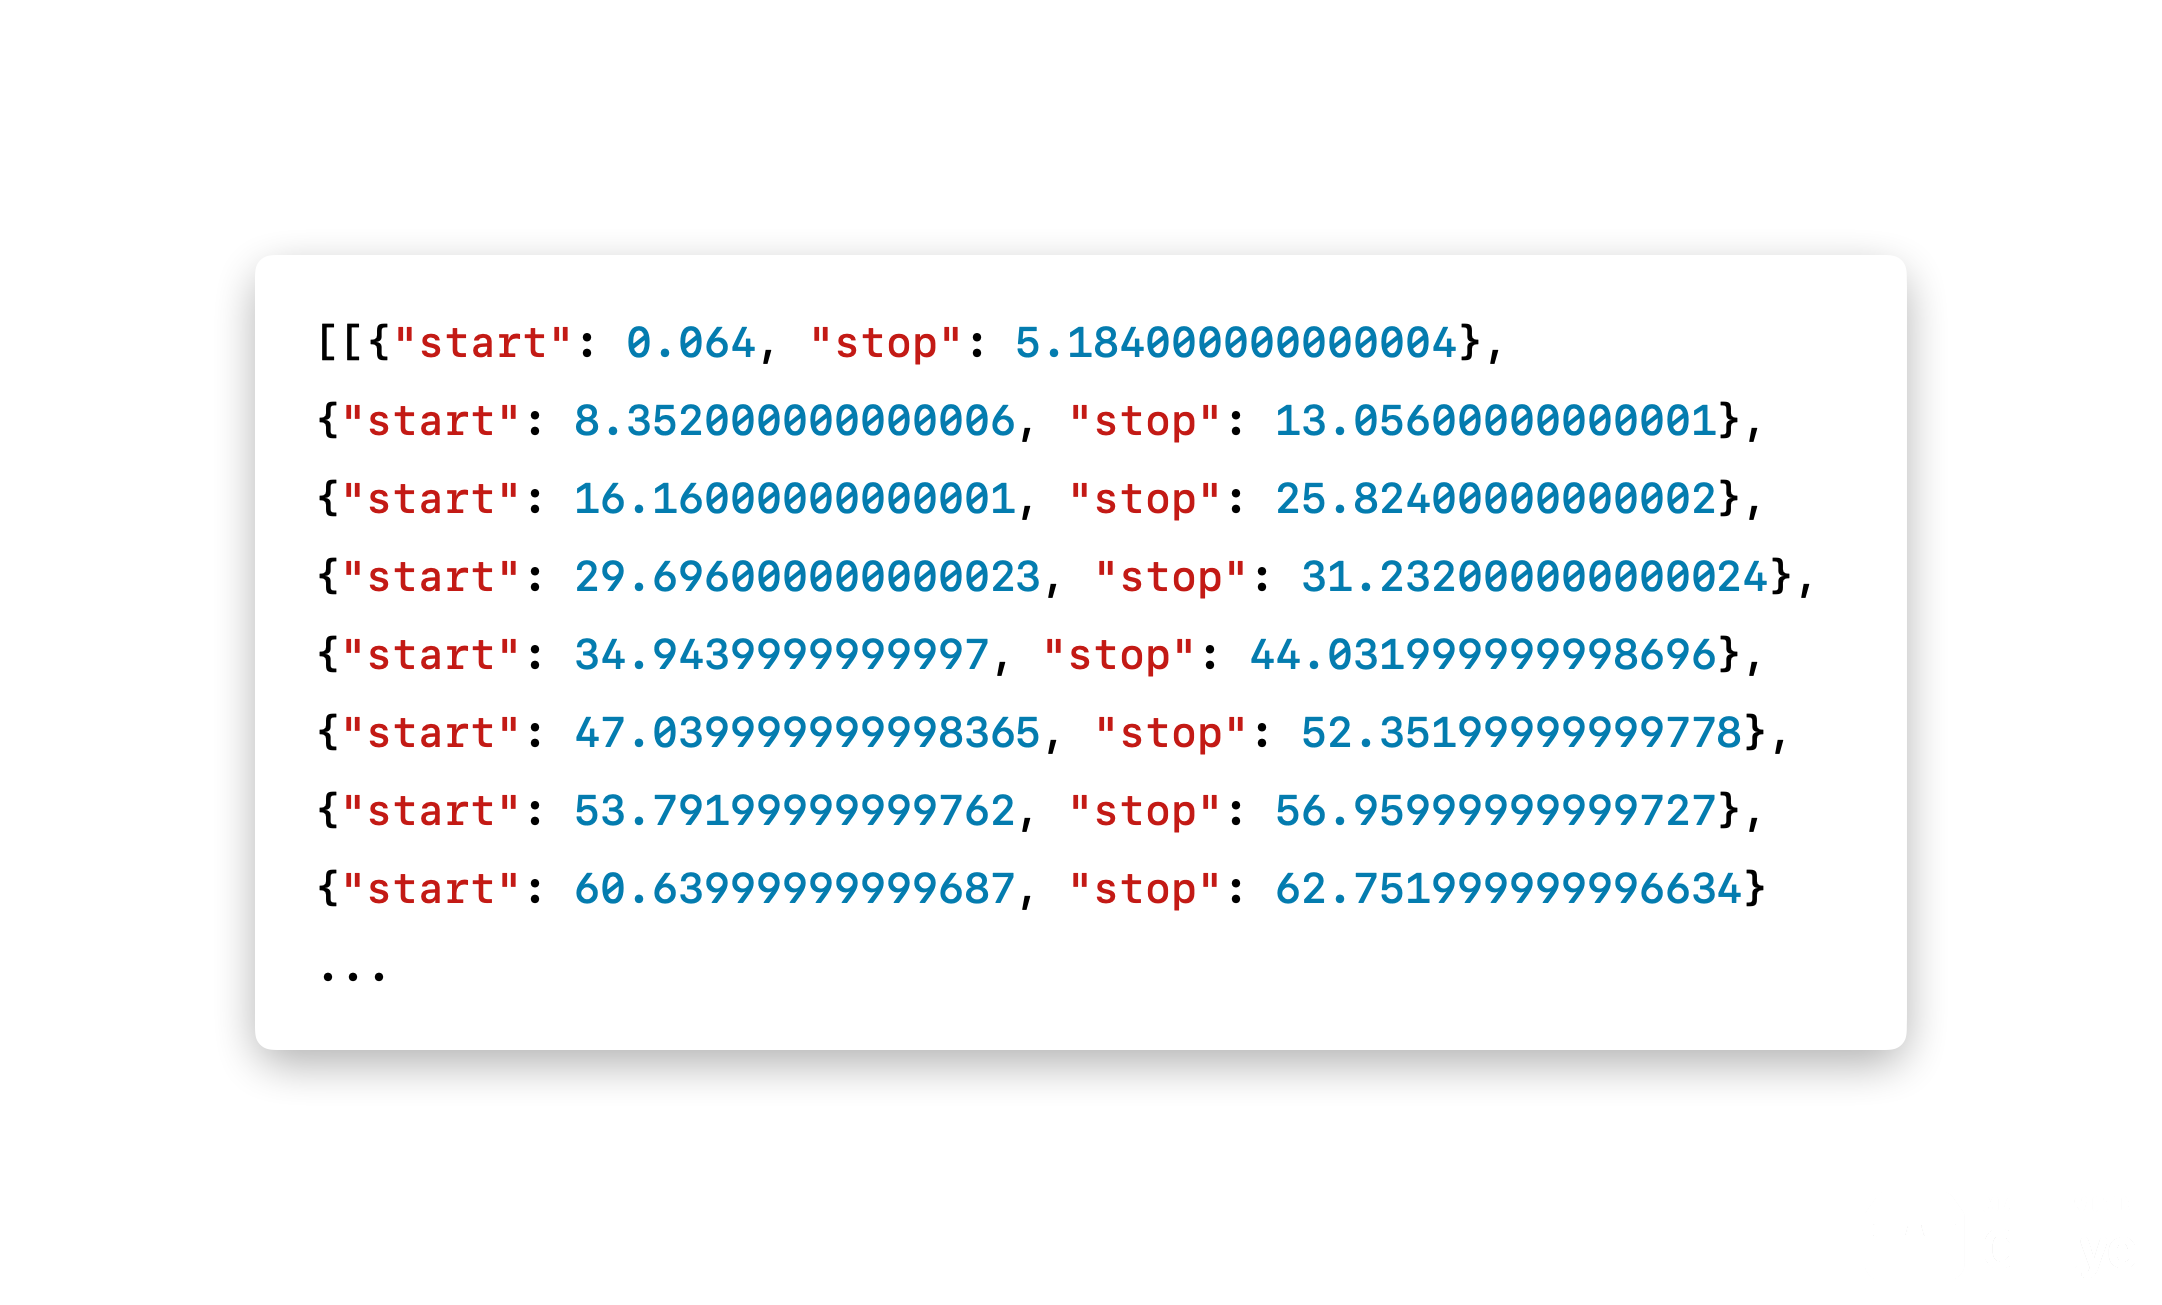
\includegraphics[width=\textwidth]{images/test-result.png}
    \caption{Test result example}
    \label{fig:test-result}
\end{figure}

From this list, in order to obtain the desired performance metrics, we need to compare it with the information contained in the metadata file. This is done checking for every millisecond of every session if it is present in the result session and in the metadata. This way we obtain the confusion matrix that we will use to obtain the metrics. Regarding the male noisy and female noisy dataset the confusion matrix and the relative performances are shown for every category of background noise always with the SNR fixed to zero. We also obtain a composite result that merges all the partial results of each category. Instead, for the noisy sessions dataset the metrics are shown for every dataset and for every SNR level.

Let's see the results of the testing and let's discuss them. A table with all the results can be found in the appendix \ref{appendix_A}.
Just to remember, the male and female noisy datasets uses a background noise with an SNR of 0db. Since we obtained all the metrics for every confidence threshold used, we decided only to show the results using the threshold that gives the best accuracy in the 'Total' category. This is the category that sums up the values of the confusion matrix of the 6 macro categories of noise used in our datasets: Nature, Domestic, Office, Public, Street and Transportation. 

Starting from the evaluation of the male noisy and female noisy datasets, in figure \ref{fig:metrics summary} we find a bar graph showing the performance metrics for both datasets using both models.   

\begin{figure}[ht]
    \centering
    \includegraphics[width=\textwidth]{images/Metrics summary.png}
    \caption{Metrics summary between the models and the datasets}
    \label{fig:metrics summary}
\end{figure}

From the graph we can see that using the silero model we obtain an accuracy of 0.87 and 0.9 for the male and female datasets, while using the webrtc model we obtain a lower accuracy of respectively 0.81 and 0.82. In particular the silero model shows slightly better values for almost every metric apart from the recall. 

To correctly compare the results of the two models we decided to obtain the ROC curve graph for both datasets. The Receiver Operating Characteristic (ROC) curve is a graphical representation used in binary classification to evaluate the performance of a model. It illustrates the trade-off between sensitivity (true positive rate) and specificity (true negative rate) across different threshold values for a model's predicted probabilities. The area under the ROC curve (AUC-ROC) is often used as a summary measure of a model's performance, with higher values indicating better discrimination ability. In figure \ref{fig:roc male} and \ref{fig:roc female} we find the ROC curves for both models and both datasets.

\begin{figure}[ht]
    \centering
    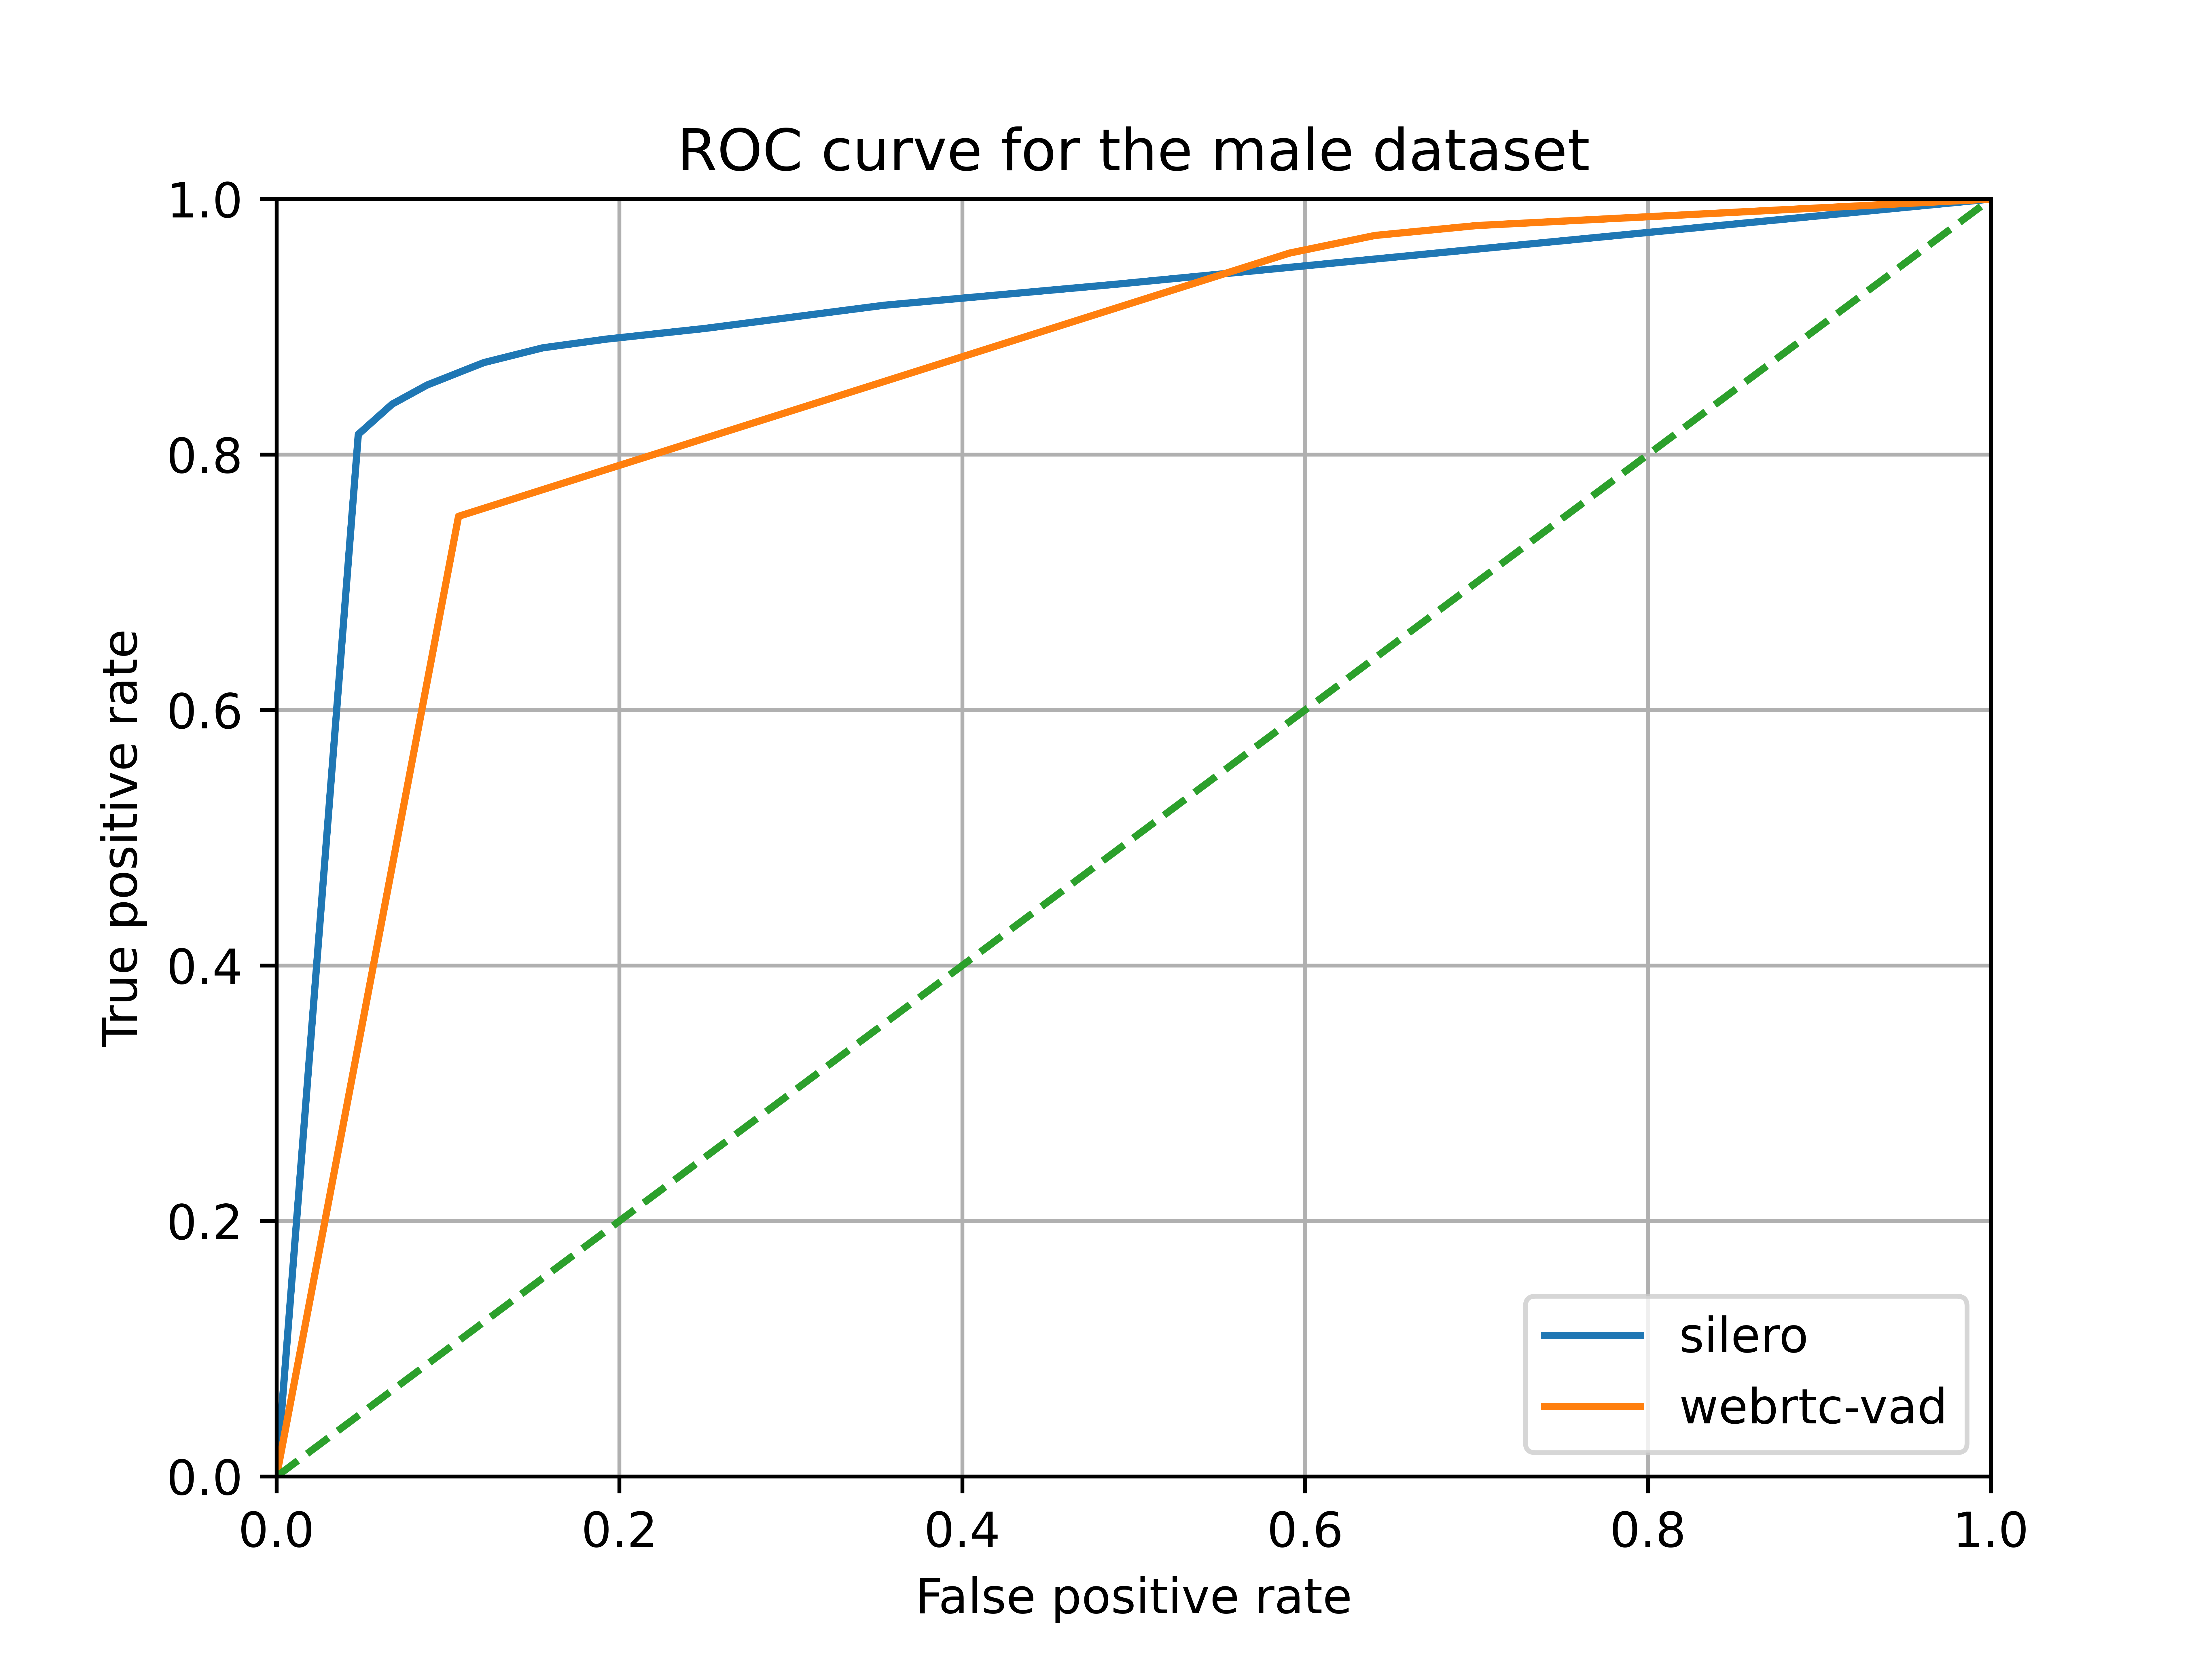
\includegraphics[width=0.8\textwidth]{images/ROC curve for the male dataset.png}
    \caption{ROC curve for the male dataset}
    \label{fig:roc male}
\end{figure}

\begin{figure}[ht]
    \centering
    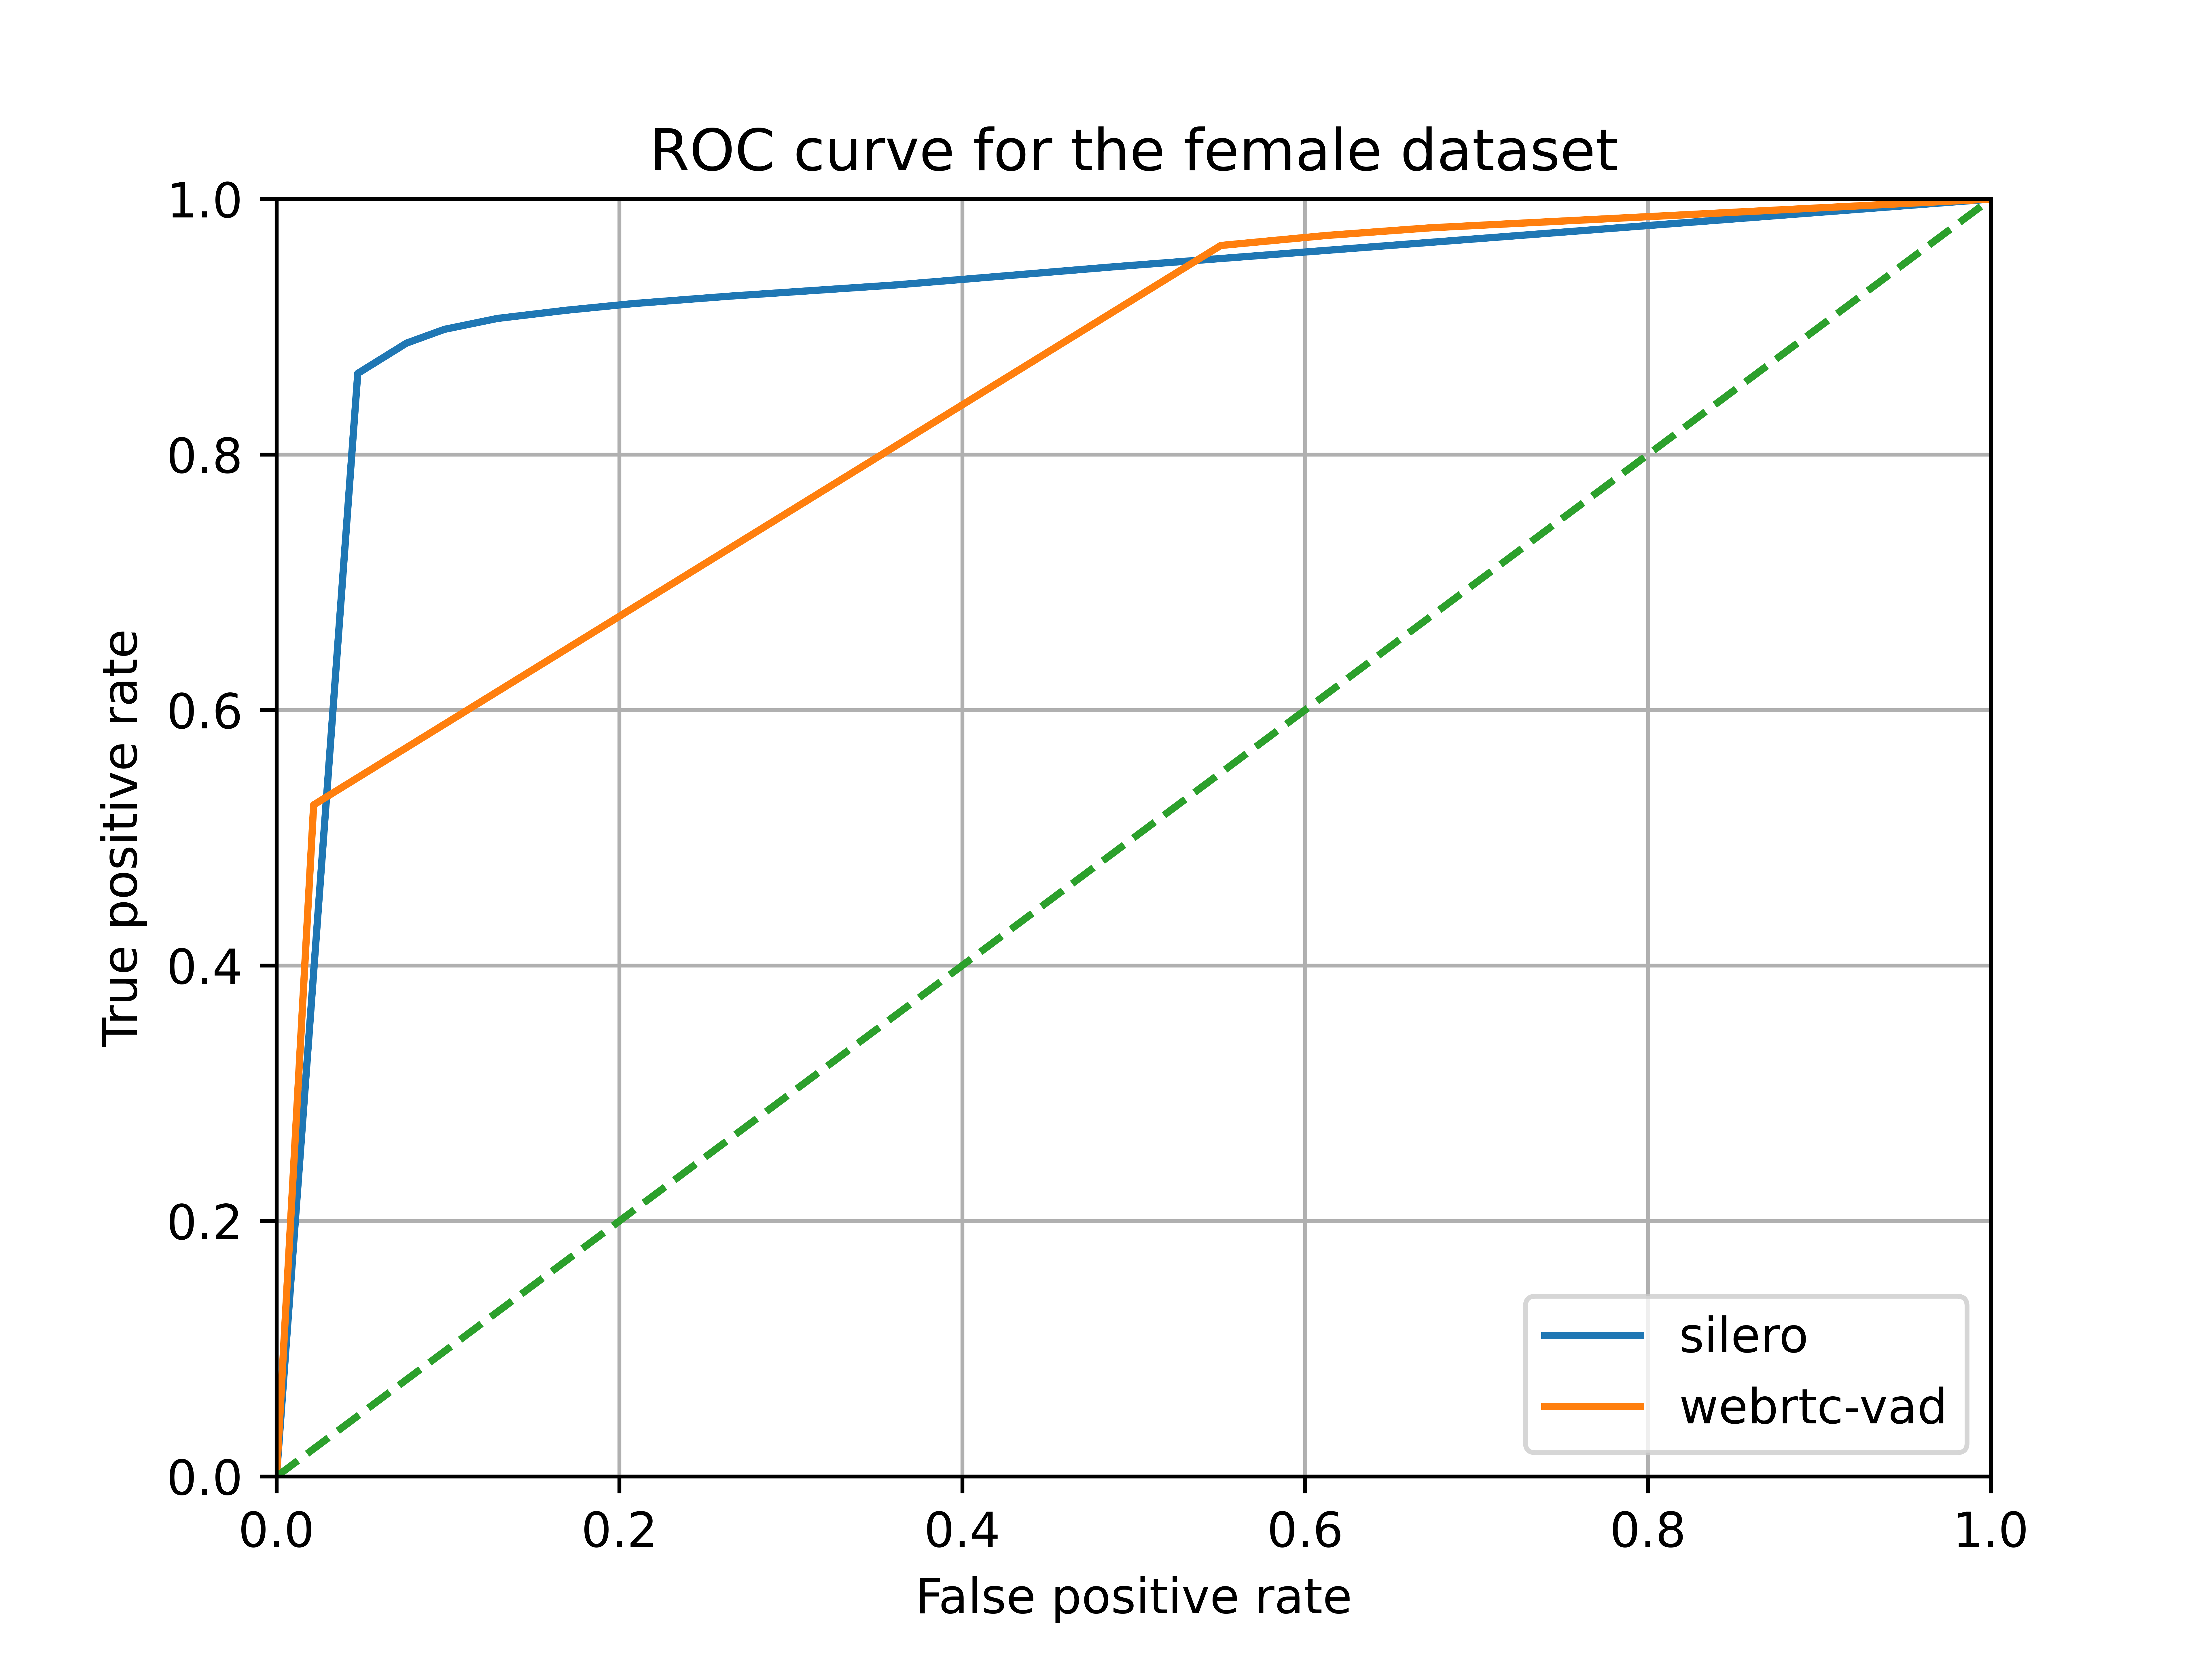
\includegraphics[width=0.8\textwidth]{images/ROC curve for the female dataset.png}
    \caption{ROC curve for the female dataset}
    \label{fig:roc female}
\end{figure}

These graphs show clearly that the silero model performs better than the webrtc model. 

Analyzing the results of the noisy sessions dataset instead we see the difference in accuracy of both models in different SNR levels of background noise. The figure \ref{fig:accuracy silero} and \ref{fig:accuracy webrtc} shows the accuracy of the silero model with the different noise categories.

\begin{figure}[ht]
    \centering
    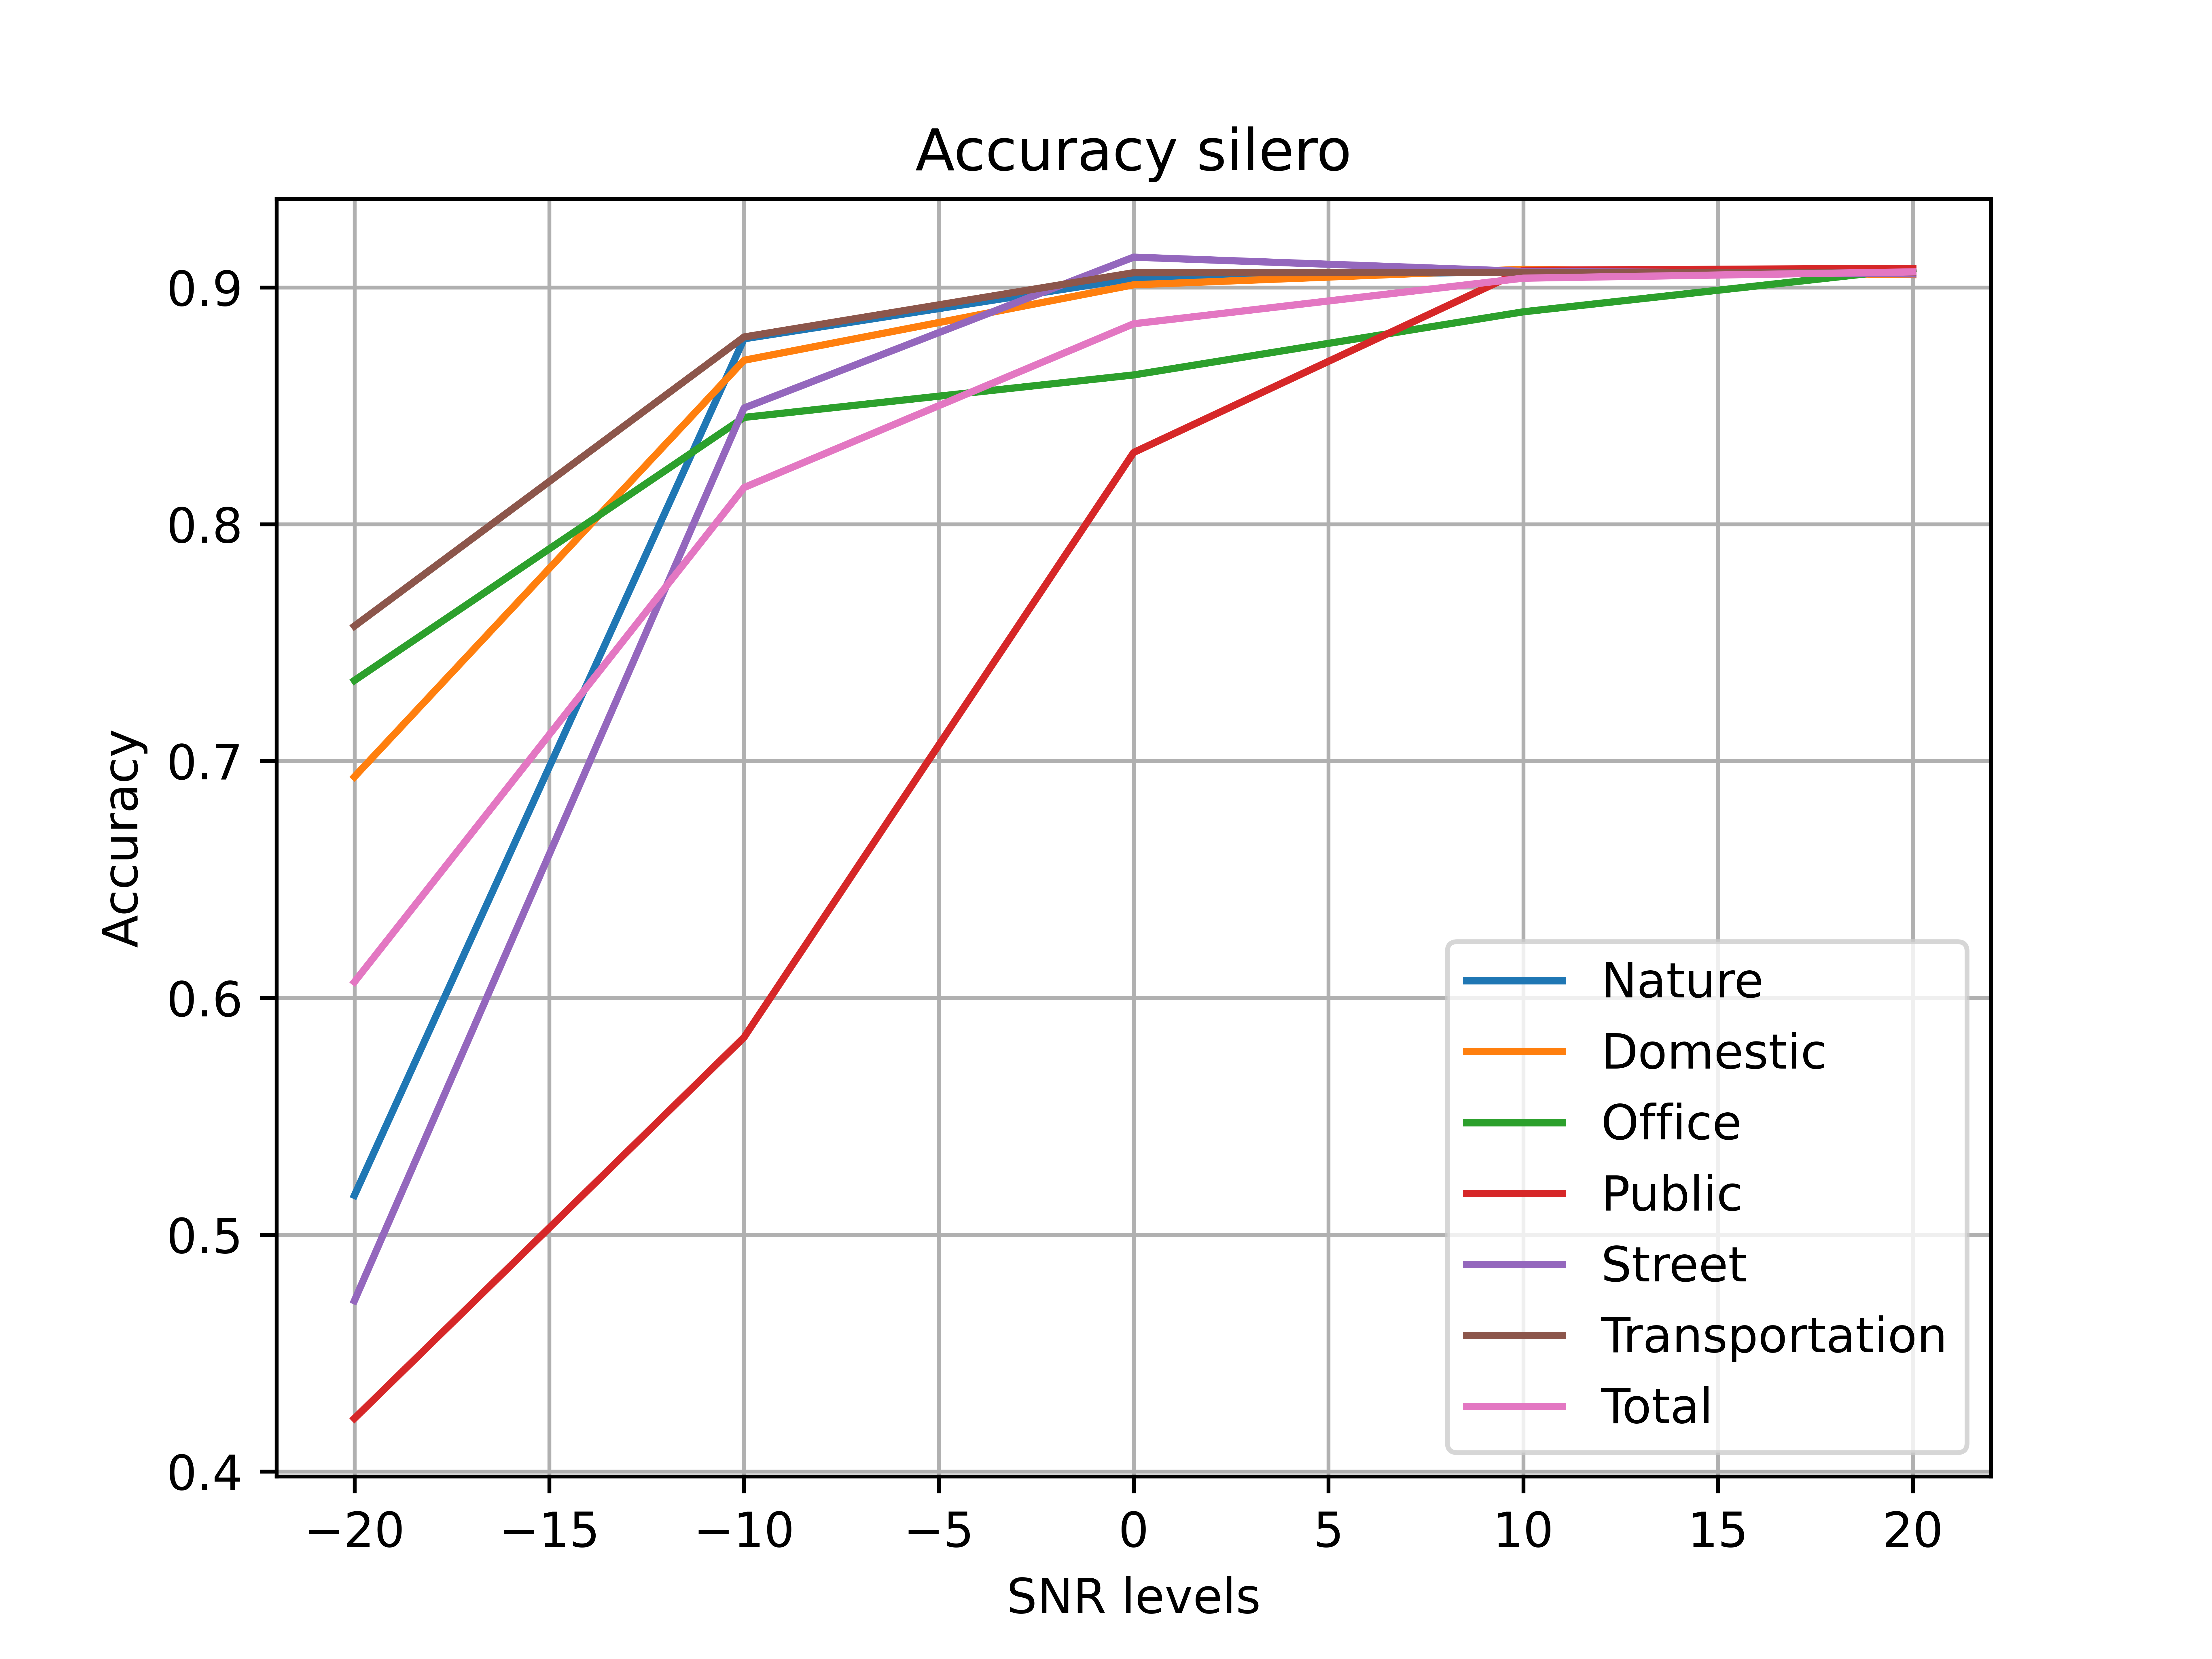
\includegraphics[width=0.8\textwidth]{images/Accuracy silero.png}
    \caption{Accuracy of the silero model with different SNR levels}
    \label{fig:accuracy silero}
\end{figure}

\begin{figure}[ht]
    \centering
    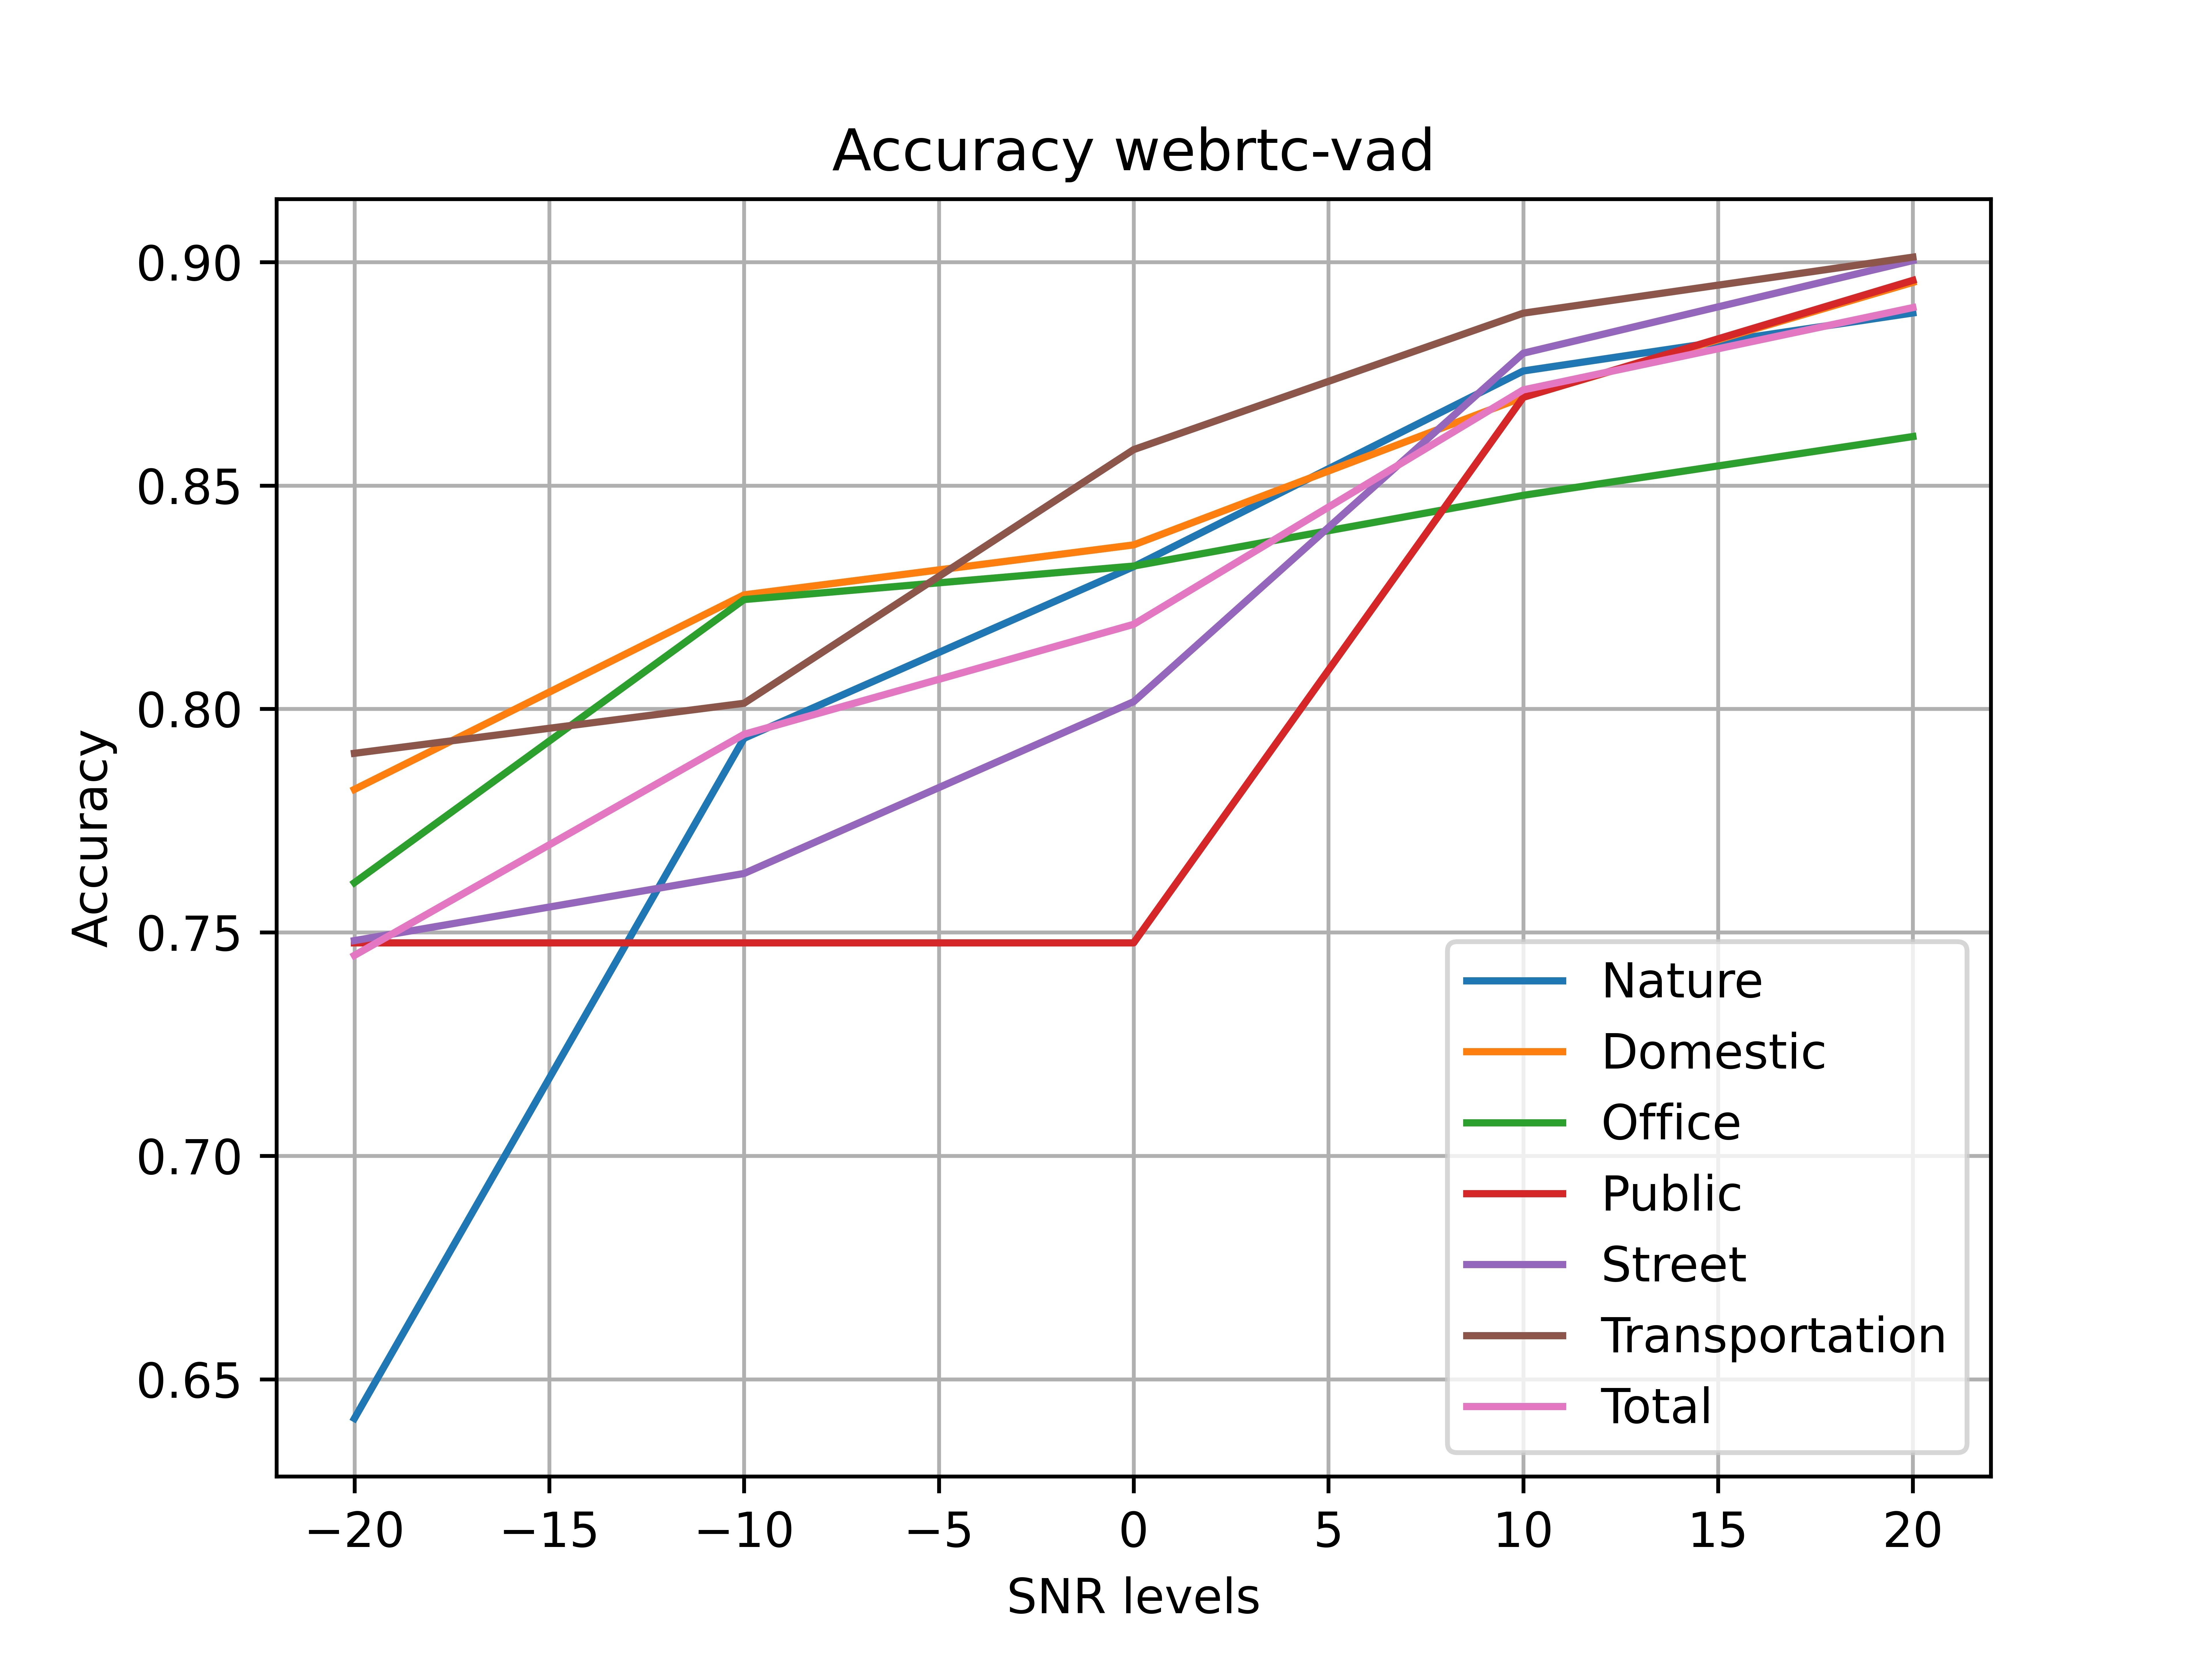
\includegraphics[width=0.8\textwidth]{images/Accuracy webrtc-vad.png}
    \caption{Accuracy of the silero model with different SNR levels}
    \label{fig:accuracy webrtc}
\end{figure}

In the end we show a direct comparison on the 'Total' categories for both models in figure \ref{fig:accuracy both models}. From the graph we can see that with higher SNR levels the models performs similarly while diminishing the SNR the silero model performs better than the webrtc model until we reach the SNR level of -10 db. Instead for the -20 db SNR the WebRTC vad performs better. The same considerations can be done for the f1-score metric. The relative graphs are shown in Figure \ref{fig:f1-score silero}, Figure\ref{fig:f1-score webrtc} and Figure \ref{fig:f1-score both models}

\begin{figure}[ht]
    \centering
    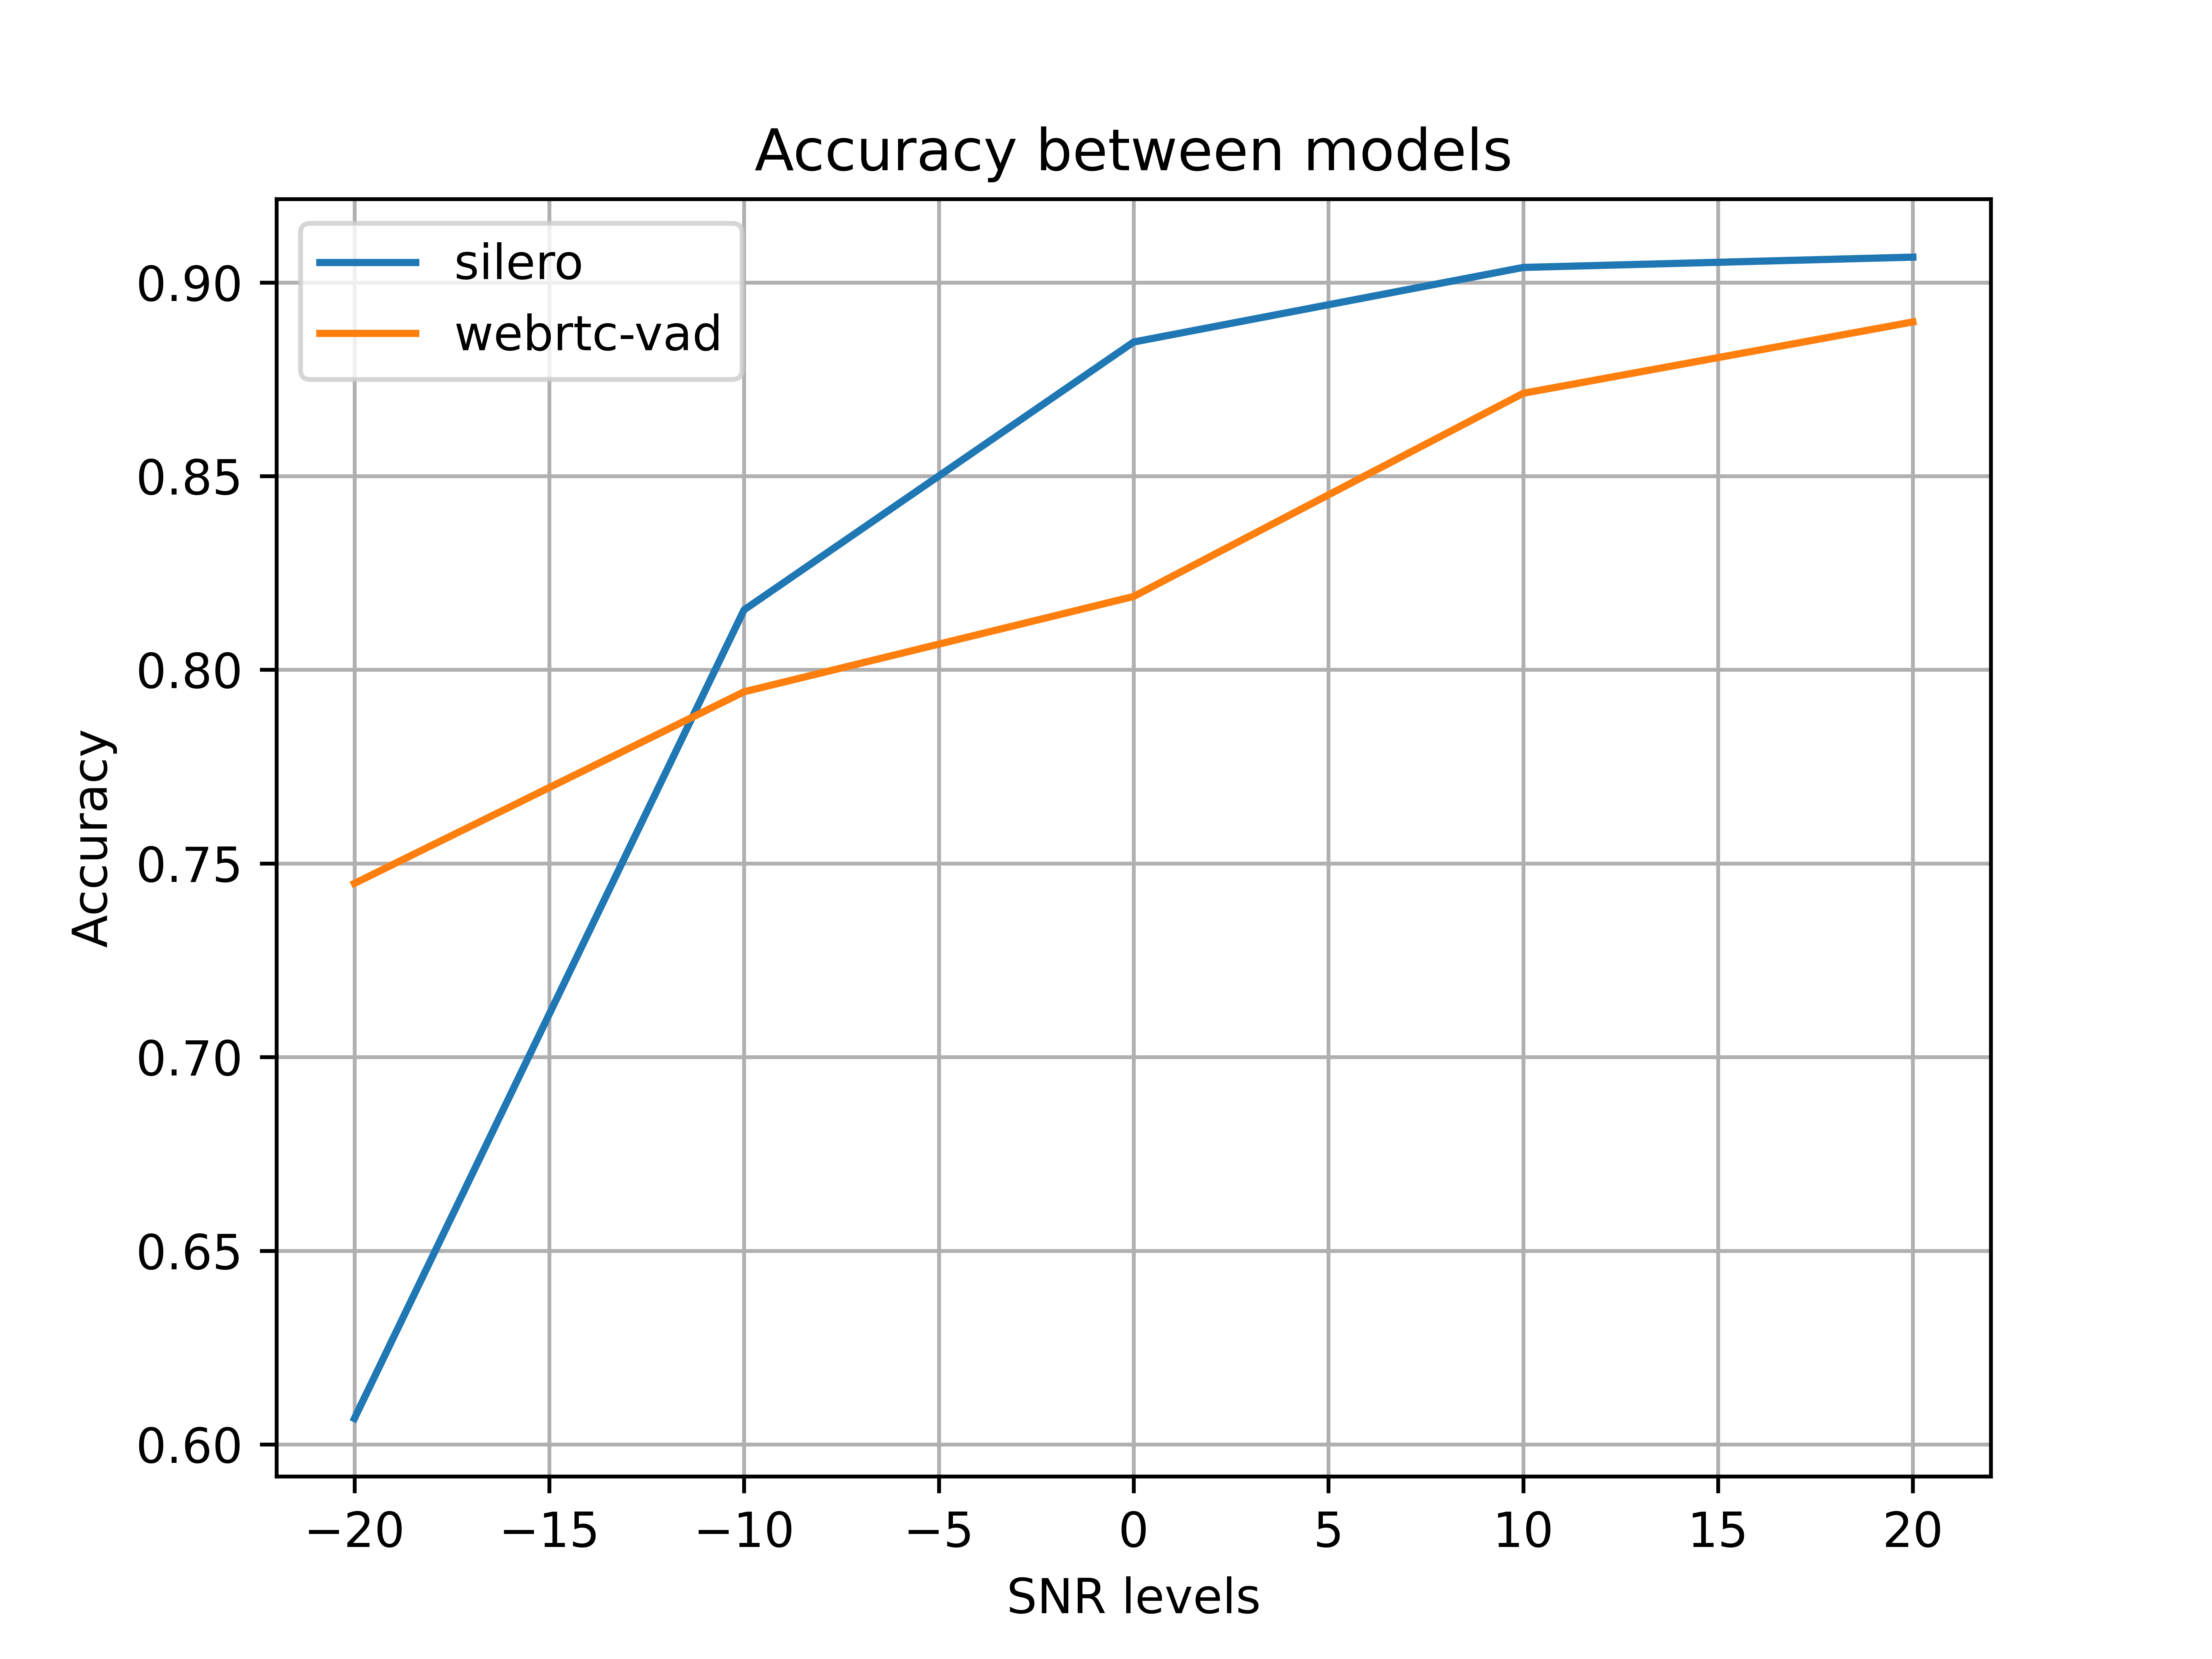
\includegraphics[width=0.8\textwidth]{images/Accuracy between models.png}
    \caption{Accuracy comparison of both models on the 'Total' category}
    \label{fig:accuracy both models}
\end{figure}

\begin{figure}[ht]
    \centering
    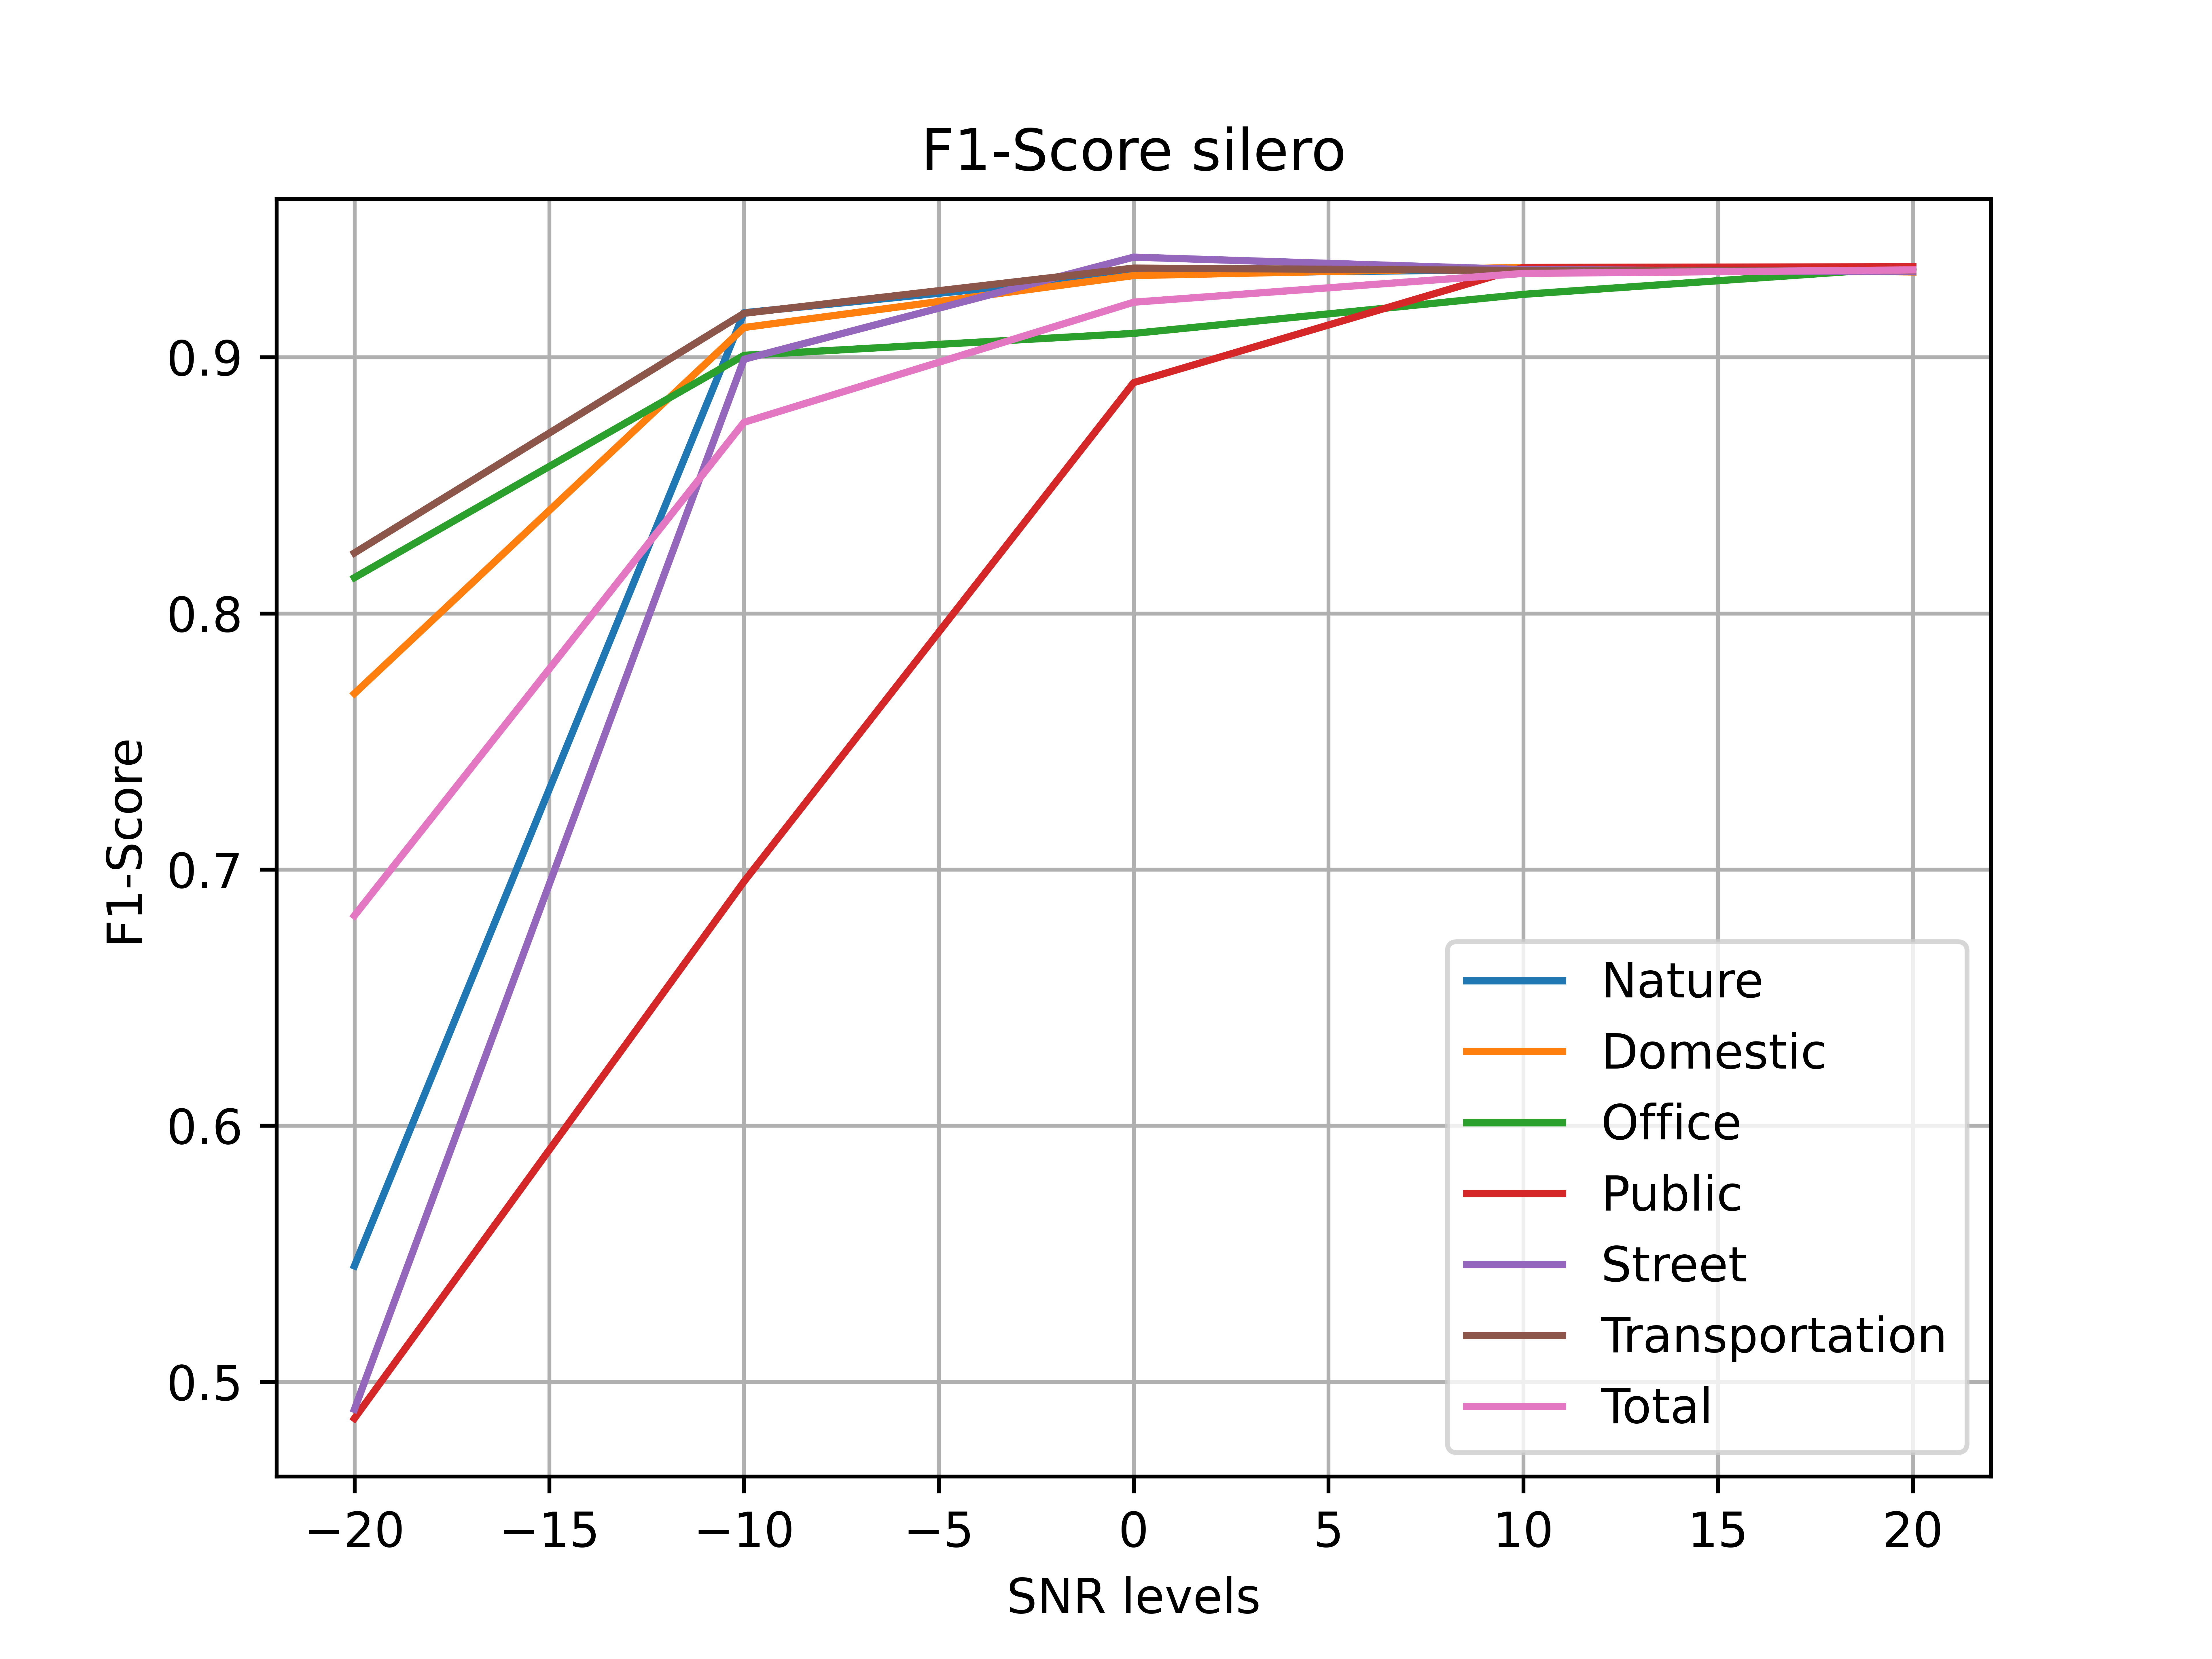
\includegraphics[width=0.8\textwidth]{images/F1-Score silero.png}
    \caption{F1-Score for the silero model with different SNR levels}
    \label{fig:f1-score silero}
\end{figure}

\begin{figure}[ht]
    \centering
    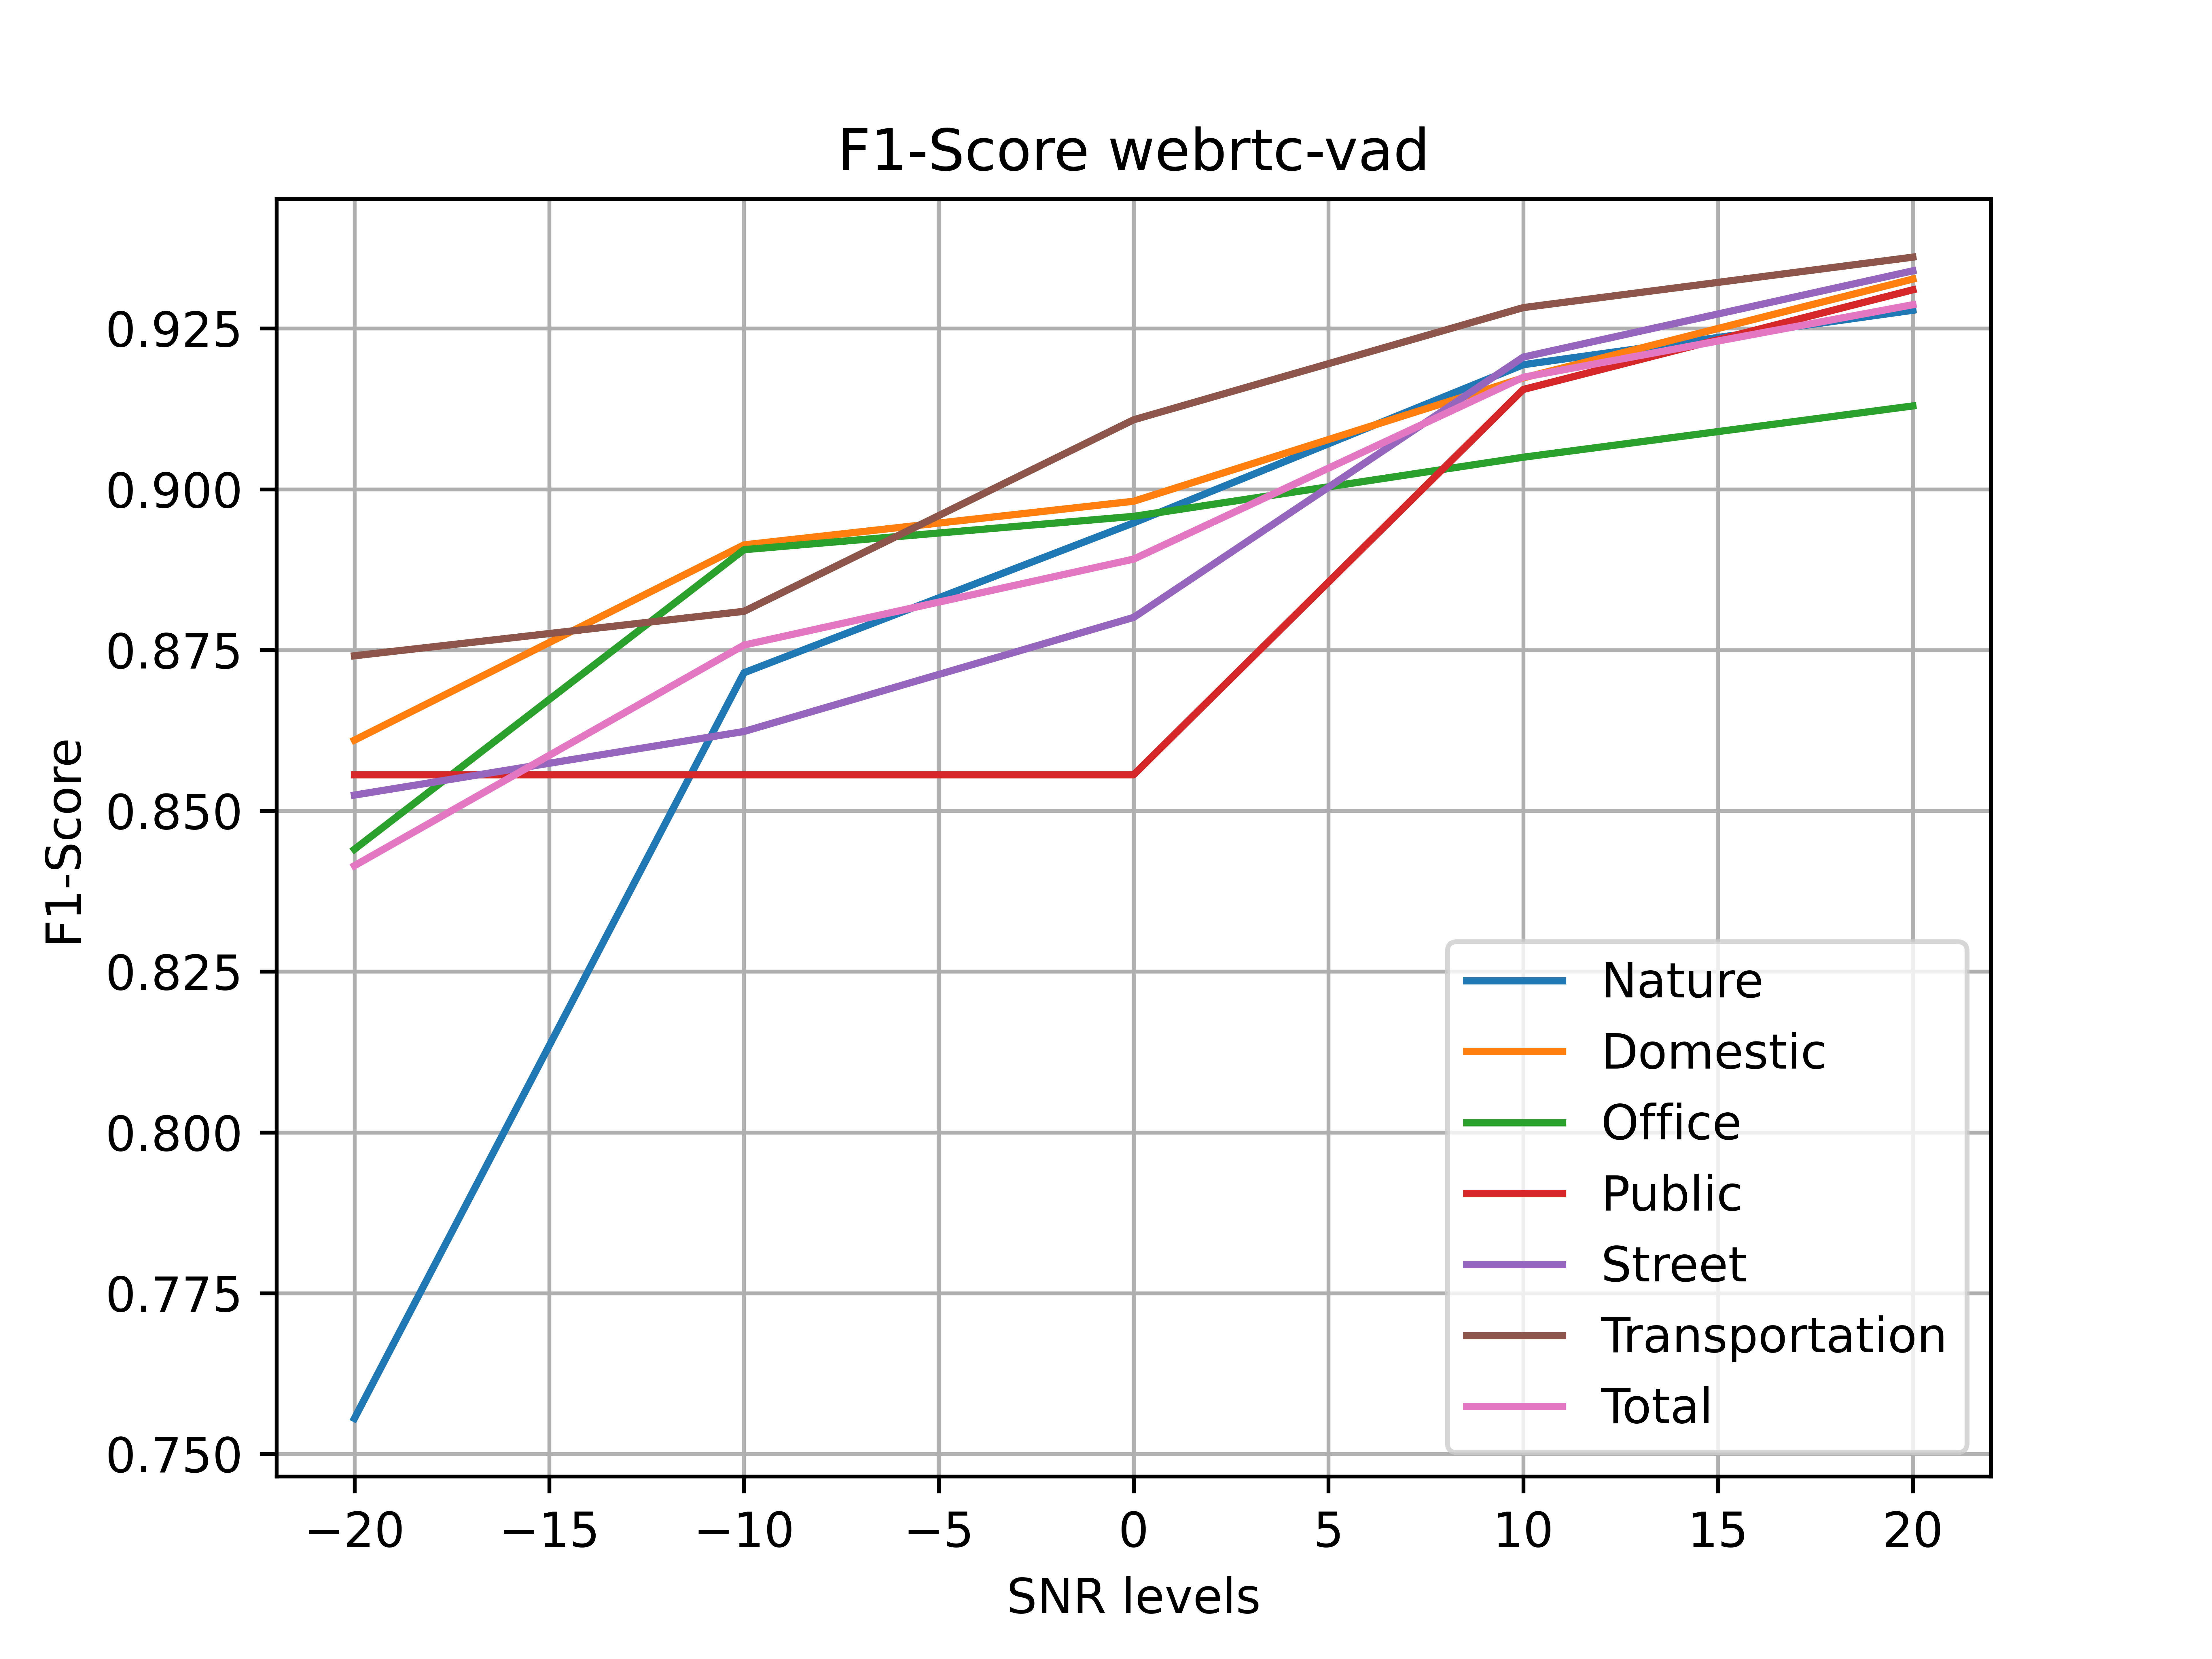
\includegraphics[width=0.8\textwidth]{images/F1-Score webrtc-vad.png}
    \caption{F1-Score for the webrtc model with different SNR levels}
    \label{fig:f1-score webrtc}
\end{figure}

\begin{figure}[ht]
    \centering
    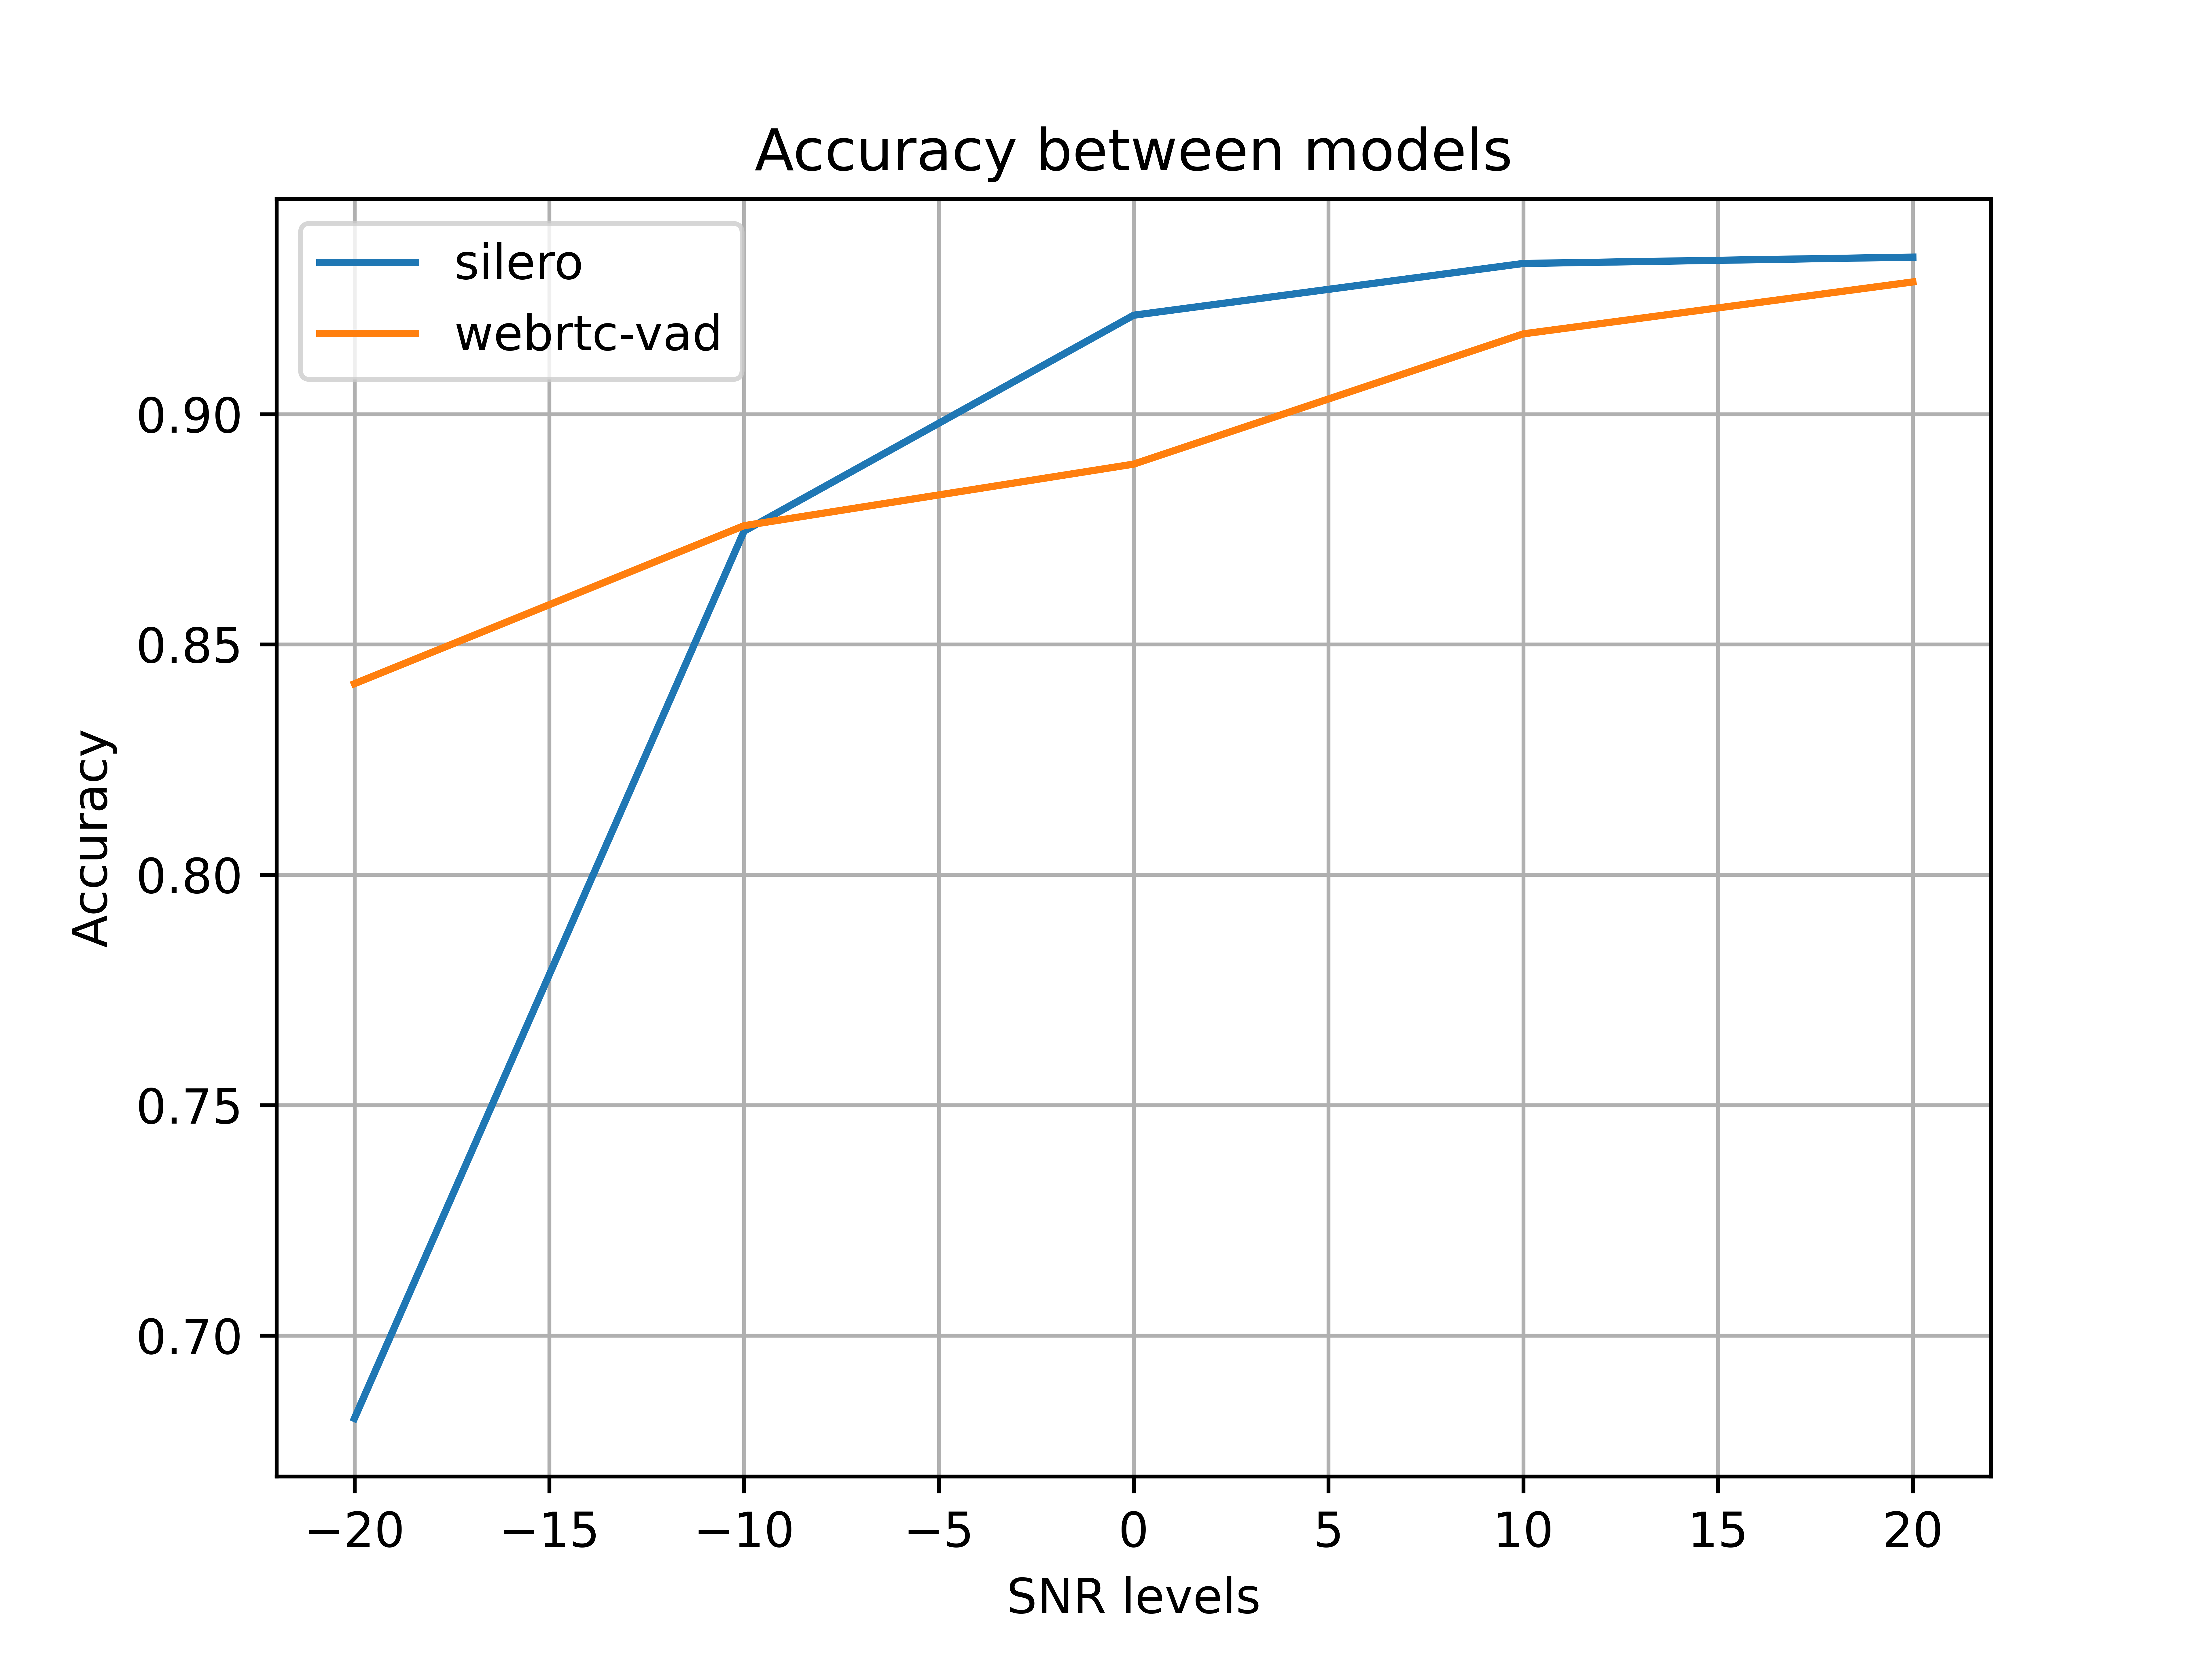
\includegraphics[width=0.8\textwidth]{images/F1-Score between models.png}
    \caption{F1-Score comparison of both models on the 'Total' category}
    \label{fig:f1-score both models}
\end{figure}

\clearpage

Finally, to comment the overall performances of the system, we can say that using the silero vad the system performs better than using the webrtc vad, especially in really noisy scenarios where the SNR is under the 0db value. The system shows good performances overall considering the really noisy scenarios, and the variability of the environment presented in the datasets, obtaining an accuracy of around 90\% that increase further when the voice is cleaner, as in the normal use case of the system.


\end{document}
